\section{Triangle}
\label{sec:Tri}

\begin{figure}[!ht]
\begin{center}
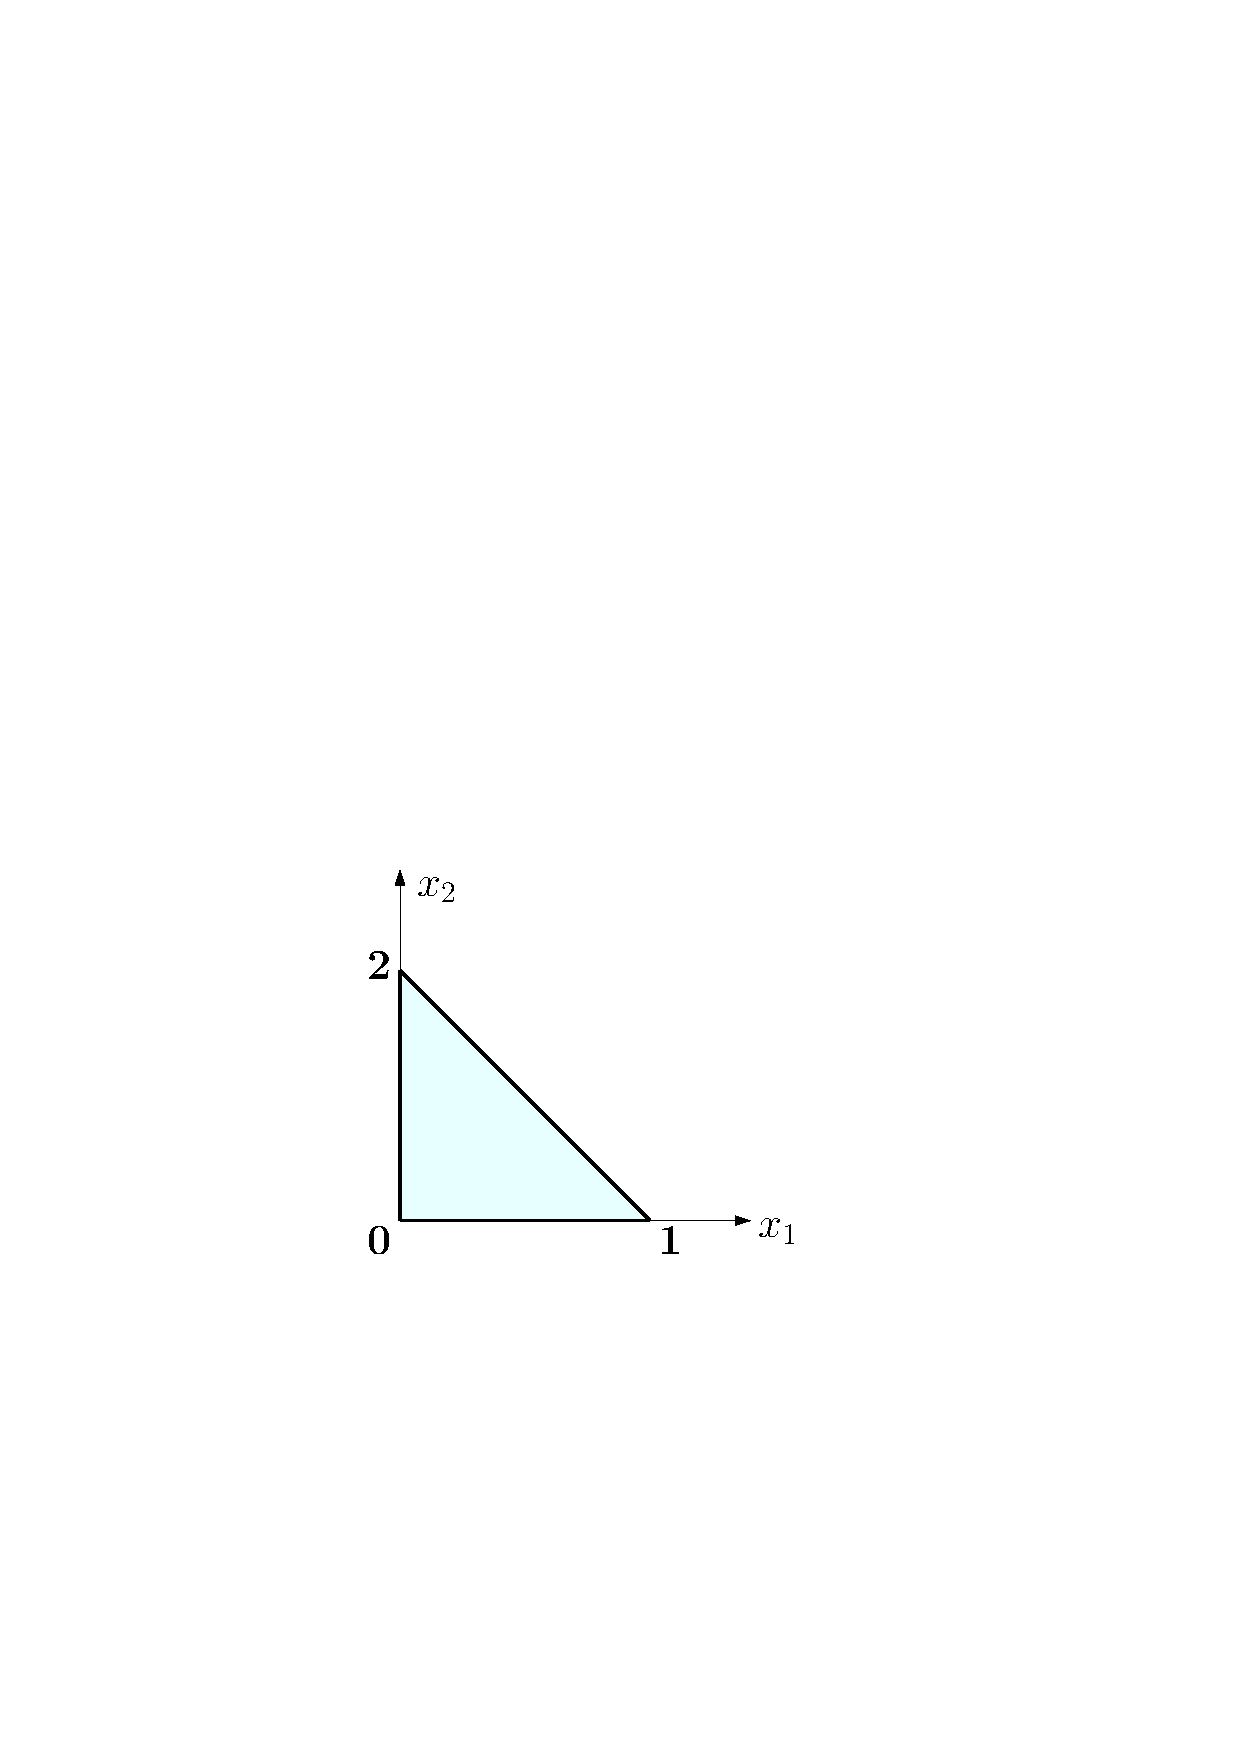
\includegraphics[scale=0.5]{./figures/MasterTri.pdf}
\caption{Master triangle with numbered vertices.}
\label{fig:MasterTriangle}
\end{center}
\end{figure}

The triangle is the 2D simplex.
The master element for triangles in the $x=(x_1,x_2)$ space is the set $\{x\in\R^2:x_1>0,x_2>0,x_1+x_2<1\}$. 
It is illustrated in Figure \ref{fig:MasterTriangle}.

Denote vertex $a$ by $v_a$, so that $v_0=(0,0)$, $v_1=(1,0)$ and $v_2=(0,1)$.
As described in \S\ref{sec:affinecoordinates}, the 2D affine coordinates, $\nu_0$, $\nu_1$ and $\nu_2$, can be easily calculated for this master triangle:
\begin{equation}
	%\begin{aligned}
	\nu_0(x)=1-x_1-x_2\,,\qquad
	\nu_1(x)=x_1\,,\qquad
	\nu_2(x)=x_2\,.
	%\begin{aligned}
\end{equation}
Their gradients are
\begin{equation}
\nabla\nu_0(x)=\Big(\begin{smallmatrix}-1\\[2pt]-1\end{smallmatrix}\Big)\,,\qquad
\nabla\nu_1(x)=\Big(\begin{smallmatrix}1\\[2pt]0\end{smallmatrix}\Big)\,,\qquad
\nabla\nu_2(x)=\Big(\begin{smallmatrix}0\\[2pt]1\end{smallmatrix}\Big)\,.
\end{equation}

Like the quadrilateral and segment, the triangle exhibits a correspondence of its vertices and its affine coordinates.
Looking at the formula $x=\nu_0(x)v_0+\nu_1(x)v_1+\nu_2(x)v_2$ this relation is evident, in the sense that each vertex is linked to \textit{one} affine coordinate (its corresponding weight).
For example $v_1$ is linked to the affine coordinate $\nu_1(x)$, and indeed it takes the value $1$ when $x=v_1$ while it is zero at the other two vertices.
%In two dimensions, we denote by $\hat\Delta$ as the master triangle. The master element is indicated in figure[]. We shall use the following notation for affine coordinates: $s_n=\nu_n$, $n\in\{0,1,2\}$ will denote affine coordinates for a triangle. Also, by ``edge 0-1'' we mean the edge defined by $\nu_0,\nu_1$. Other edges are similarly defined. Observe that
%\be
%\sum_{n=0}^2 \nu_n( x)=1\,,
%\ee
%and
%\be
%\nu_n( x)\ge0\,,
%\ee
%for all $ x\in\hat\Delta$.

\subsubsection*{Exact Sequence}


%Also, $(\mathcal{P}^p)^2=\mathcal{P}^p\times\mathcal{P}^p$ and similarly with $(\tilde{\mathcal{P}}^p)^2$.

%i.e., vector space of 2-tuples of elements in $\mathcal{P}^p$. Furthermore, define $\tilde{\mathcal{P}}^{p} = \tilde{\mathcal{P}}^{p} (\hat\Delta)$ to be the subspace of homogeneous polynomials of order $p$ on $\hat\Delta$. The space $\left(\tilde{\mathcal{P}}^{p}\right)^2$ is defined similarly.

%It is our intent to reproduce the\footnote{%Given the 2D rotation $R:(x_1,x_2)\mapsto(x_2,-x_1)$, observe that $R:H(\text{curl}) \to H(\text{div})$ is an isomorphism. Moreover, $\nabla\times = R\nabla$, $\text{curl}(\,\cdot\,) = \nabla\cdot R(\,\cdot\,)$.
%NEW FOOTNOTE. REFERENCE INTRODUCTION.} 2D exact sequence(s)

As with the quadrilateral, the triangle will have 2D discrete polynomial exact sequences that represent the continuous exact sequence \eqref{eq:2DExactSeq} and its rotated analogue \eqref{eq:2DExactSeqRotated}. 
They are
%\begin{equation}
%\begin{alignedat}{4}
%    &W^{p} \xrightarrow{\,\,\nabla\,\,} &Q^{p} \xrightarrow{\nabla\times} &&Y^{p} \,,\\
%    &W^{p} \xrightarrow{\mathrm{curl}\,} &V^{p} \xrightarrow{\,\nabla\cdot\,} &&Y^{p} \,,
%\end{alignedat}
%\end{equation}
%where more specifically the spaces \citeyearpar{Nedelec80} of the first type for the quadrilateral are utilized:
%\begin{equation}
%    \begin{aligned}
%    W^{p,q} & = \mathcal{Q}^{p,q}= \mathcal{P}^p(\xi_1)\otimes \mathcal{P}^q(\xi_2)\,, \\
%    Q^{p,q} & = \mathcal{Q}^{p-1,q} \times\mathcal{Q}^{p,q-1}\,, \\
%    V^{p,q} & = \mathcal{Q}^{p,q-1} \times\mathcal{Q}^{p-1,q}\,, \\
%    Y^{p,q} & = \mathcal{Q}^{p-1,q-1}\,.
%    \end{aligned}
%\end{equation}
%
%Let $\mathcal{P}^p =\mathcal{P}^p(x_1,x_2)$ be the space of polynomials of total order $p$ in the $x=(x_1,x_2)$ space. 
%Recall the 2D exact sequence for simply connected domains \eqref{eq:2DExactSeq} and its rotated analogue \eqref{eq:2DExactSeqRotated}:
%\begin{equation}
%\begin{alignedat}{4}
%	&H^1 \xrightarrow{\,\,\nabla\,\,} &&H(\mathrm{curl}) \xrightarrow{\nabla\times} \,&L^2 \,,\\
%	&H^1 \xrightarrow{\mathrm{curl}\,}\, &&H(\mathrm{div})\, \xrightarrow{\,\,\nabla\cdot\,\,} &L^2 \,.
%\end{alignedat}
%\end{equation}
%
%The corresponding polynomial exact sequences are
\begin{equation}
\begin{alignedat}{4}
    &\mathcal{P}^p \xrightarrow{\,\,\nabla\,\,} &\mathcal{N}^p \xrightarrow{\nabla\times} && \mathcal{P}^{p-1} \,,\\
    &\mathcal{P}^p \xrightarrow{\mathrm{curl}\,} &\mathcal{RT}^p \xrightarrow{\,\nabla\cdot\,} &&\mathcal{P}^{p-1} \,,
    \label{eq:EStriangle}
\end{alignedat}
\end{equation}
where $\mathcal{P}^p =\mathcal{P}^p(x_1,x_2)$ is the space of polynomials of total order $p$.
The spaces $\mathcal{N}^p$ and $\mathcal{RT}^p$ are the N\'{e}d\'{e}lec and Raviart-Thomas spaces for simplices:
\begin{align}
	\label{eq:NedelecSpace}
	\mathcal{N}^p&=(\mathcal{P}^{p-1})^N\oplus\Big\{E\in(\tilde{\mathcal{P}}^{p})^N: x\cdot E(x)=0\,\text{ for all } x\in\R^N\Big\}\,,\\
	\label{eq:RaviartThomasSpace}
	\mathcal{RT}^p&=(\mathcal{P}^{p-1})^N\oplus\Big\{V\in(\tilde{\mathcal{P}}^{p})^N: V(x)=\phi(x)x
		\, \text{ with }\phi\in\tilde{\mathcal{P}}^{p-1}\,\text{ and }x\in\R^N\Big\} \,.
\end{align}
In the case of the triangle, the number of spatial dimensions is $N=2$.
%, and in fact $\mathcal{N}^p$ and $\mathcal{RT}^p$ are ``rotations'' of each other.
%That is, $\mathcal{RT}^p=\{V=\Big(\begin{smallmatrix}0&1\\[2pt]-1&0\end{smallmatrix}\Big)E=: E\in\mathcal{N}^p\}$
Note the sequence has an overall drop in polynomial order of one. 
This makes it compatible with the construction presented for the quadrilateral.
Moreover, all of the spaces in the exact sequences above are invariant under affine transformations. 
This implies the exact sequence takes the same form for any given triangle (provided it is mapped via an affine transformation from the master triangle, which is always possible).
%That is, the pullback of an affine transformation brings $\mathcal{N}^p(\hat\Delta)$ onto $\mathcal{N}^p(\Delta)$, etc. Here, $\Delta$ denotes the triangle in physical space (i.e., the physical element).

\subsection{\texorpdfstring{$H^1$}{H1} Shape Functions}
%In two dimensions, the trace of $H^1$ functions is the value of the function itself along the boundary.
%Hence, all vertex functions vanish at all nonadjacent edges, and all edge functions should vanish at all other edges.
%The bubbles will vanish at all edges.

All shape functions defined here will lie in $\mathcal{P}^{p}$, which has dimension $\frac{1}{2}(p+2)(p+1)$. 
Moreover, a careful count of the linearly independent shape functions will coincide with that dimension, so that indeed the space is spanned.

\subsubsection{\texorpdfstring{$H^1$}{H1} Vertices}
%Affine coordinates in two dimensions will be denoted by $\nu_0$, $\nu_1$ and $\nu_2$. They are written explicitly for our master triangle:
%\begin{equation}
%	%\begin{aligned}
%	\nu_0(x)=1-x_1-x_2\,,\qquad
%	\nu_1(x)=x_1\,,\qquad
%	\nu_2(x)=x_2\,.
%	%\begin{aligned}
%\end{equation}
%Their gradients are
%\begin{equation}
%\nabla\nu_0(x)=\Big(\begin{smallmatrix}-1\\[2pt]-1\end{smallmatrix}\Big)\,,\qquad
%\nabla\nu_1(x)=\Big(\begin{smallmatrix}1\\[2pt]0\end{smallmatrix}\Big)\,,\qquad
%\nabla\nu_2(x)=\Big(\begin{smallmatrix}0\\[2pt]1\end{smallmatrix}\Big)\,.
%\end{equation}
%Take note of the above, since they will be used explicitly or implicitly in the computations of shape functions throughout this section.

In this case, for a given vertex, the associated shape function will be its related affine coordinate.
For example, $v_0$ is linked to $\nu_0(x)$, so its associated vertex function is simply 
\begin{equation*}
	\phi^\mathrm{v}(x)=\nu_0(x)\,.
\end{equation*}
As expected, it vanishes at the disjoint opposite edge 12 and its trace over the adjacent edges is a 1D $H^1$ vertex function associated to the vertex. 
Indeed, the traces are explicitly,
\begin{equation*}
	\nu_0(x)|_{x_2=0}=1-x_1=\mu_0(x_1)\,,\qquad\nu_0(x)|_{1-x_1-x_2=0}=0\,,\qquad\nu_0(x)|_{x_1=0}=1-x_2=\mu_0(x_2)\,. 
\end{equation*}
Lastly, the function decays linearly and is in the lowest order possible space, $\mathcal{P}^1$, so that it respects the hierarchy in $p$.

In general, the vertex functions and their gradient are,
\begin{equation}
    \phi^\mathrm{v}(x)=\nu_a(x)\,,\qquad\quad\nabla\phi^\mathrm{v}(x)=\nabla\nu_a(x)\,,
\end{equation}
for $a=0,1,2$.
There are a total of $3$ vertex functions (one for each vertex).
%
%
%The $H^1$ vertex shape functions will precisely be these affine coordinates. 
%They are presented next with their gradients
%\begin{equation}
%	\phi^\mathrm{v}(x)=\nu_a(x)\,,\qquad\nabla\phi^\mathrm{v}(x)=\nabla\nu_a(x)\,,\qquad a=0,1,2\,.
%\label{eq:H1_CountingSimplexVert}
%\end{equation}
%Clearly the vertex shape functions vanish at all vertices except vertex $a$ for $a=0,1,2$. By linearity, their trace is of the right form. That is, it satisfies the vanishing properties and is compatible with the vertex functions of the segment (and thus with edges of the quadrilateral). Take for example vertex 0 which has vertex function $\nu_0(x)$. The traces are
%\begin{equation*}
%	\nu_0(x)|_{x_2=0}=1-x_1=\mu_0(x_1)\,,\qquad\nu_0(x)|_{x_2=1-x_1}=0\,,\qquad\nu_0(x)|_{x_1=0}=1-x_2=\mu_0(x_2)\,, 
%\end{equation*}
%so that the function vanishes at the only (opposite) nonadjacent edge, and it has the form $\mu_b(x_a)$ for some $a=1,2$ and $b=0,1$ for the other two edges (which are compatible with the segment vertex functions).

\subsubsection{\texorpdfstring{$H^1$}{H1} Edges}
\label{sec:H1edgesTri}

For the construction of the edge functions consider edge 01 as an example.
To satisfy compatibility with the quadrilateral, the shape functions should have $\phi_i^\E(\vec{\mu}_{01}(x_1))$ as the trace over edge 01, and be zero at the two other edges.
Additionally, they should be polynomial (they should be in $\mathcal{P}^p$).

Unfortunately, at first sight the construction is not trivial since many intuitive approaches lead to violating some of the required properties mentioned above.
This is in large part due to the fact that the triangle is \textit{not} a Cartesian product of lower dimensional elements.
Luckily, these issues are all solved by the process of homogenization, which is viewed as a particular extension of the lower dimensional edge functions $\phi_i^\E(\vec{\mu}_{01}(x_1))$.
The idea is to exploit the 2D \textit{triangle} affine coordinates associated to edge 01, which are $\nu_0$ and $\nu_1$ (those linked to the vertices $v_0$ and $v_1$ which compose the edge).
Indeed, let the shape functions for this edge be
\begin{equation*}
    \phi_i^\mathrm{e}(x)=\phi_i^\E(\vec{\nu}_{01}(x))=[L_i](\vec{\nu}_{01}(x))
    	=(\nu_0(x)+\nu_1(x))^i
    		[L_i]\Big(\textstyle{\frac{\nu_0(x)}{\nu_0(x)+\nu_1(x)}},\textstyle{\frac{\nu_1(x)}{\nu_0(x)+\nu_1(x)}}\Big)\,,
\end{equation*}
with $i=2,\ldots,p$.
Here, property \eqref{eq:ScalingProperty} was used.
Notice that $\nu_2=0$ is the equation for edge 01 and similarly with the other edges.
Hence, using the vanishing properties of $\phi_i^\E$ in \eqref{eq:phiEvanishing}, it follows that the trace properties are satisfied:
\begin{alignat*}{3}
    &\phi_i^\mathrm{e}(x)|_{x_2=0}&&=\phi_i^\E(\vec{\nu}_{01}(x))|_{\nu_2=0}=\phi_i^\E(\vec{\mu}_{01}(x_1))\,,\\
    &\phi_i^\mathrm{e}(x)|_{1-x_1-x_2=0}&&=\phi_i^\E(\vec{\nu}_{01}(x))|_{\nu_0=0}=\phi_i^\E(0,\mu_1(x_1))=0\,,\\
  	&\phi_i^\mathrm{e}(x)|_{x_1=0}&&=\phi_i^\E(\vec{\nu}_{01}(x))|_{\nu_1=0}=\phi_i^\E(\mu_0(x_2),0)=0\,.
\end{alignat*}
In this case, the decay of each shape function is represented by the nonlinear function $(\nu_0(x)+\nu_1(x))^i$, which comes hidden within the homogenization.
Additionally, $\phi_i^\E(\vec{\nu}_{01})\in\tilde{\mathcal{P}}^i(\nu_0,\nu_1)$ by homogenization while $\nu_0(x),\nu_1(x)\in\mathcal{P}^1(x)$, meaning that the edge functions $\phi_i^\E(\vec{\nu}_{01}(x))$ are in $\mathcal{P}^i(x)\subseteq\mathcal{P}^p(x)$ as required.
%To construct these edge functions one must be aware that the trace over the other two edges should vanish, while the trace over the edge itself should have the correct form compatible with the segment edge bubbles. 
%That is, the trace should be of the form $L_i$ for the given edge. 
%
%This amounts to starting with $L_i$ over the given edge and then choosing a correct blending function which extends (or lifts) it to the rest of the element, while respecting the vanishing conditions. 
%This extension should also be polynomial (it should be in $\mathcal{P}^p$). 
%Fortunately, all these criteria are met by the process of \textit{homogenization} (see \textit{cite homog}).
%
%To see this, take for example edge 01, and the related affine coordinates $\nu_0$ and $\nu_1$. Notice their restriction to edge 01 is of the form 
%\begin{equation*}
%	\nu_0(x)|_{x_2=0}=\mu_0(x_1)\,,\qquad\quad \nu_1(x)|_{x_2=0}=\mu_1(x_1)\,.
%\end{equation*}
%This might suggest a similar approach to the quadrilateral at first, where one seeks to work with 1D affine coordinates and a linear blending function. 
%However, attempts show that there is no easy fix. 
%This is due to the fact that the triangle is \textit{not} a tensor product of two line segments. 
%Indeed, ideally one should try to exploit the geometry by using the 2D affine coordinates directly.
%Following \textit{cite Sch\"{o}berl}, this can be achieved by a proper scaling of the original polynomial.
%In the context of this work, this process is called homogenization and results in
%\begin{equation*}
%	[L_i](\nu_0,\nu_1)=L_i(\nu_1;\nu_0+\nu_1)
%	=\underbrace{(\nu_0+\nu_1)^i}_{\text{blend}}
%		\underbrace{L_i(\underbrace{\textstyle{\frac{\nu_1}{\nu_0+\nu_1}}}_{\text{project}})}_{\text{evaluate}}\,.
%\end{equation*}
%By construction, $[L_i](\nu_0,\nu_1)$ is homogeneous in $\nu_0$ and $\nu_1$ of total order $i$, so that $[L_i](\nu_0(x),\nu_1(x))\in\mathcal{P}^i$. 

\begin{figure}[!ht]
\begin{center}
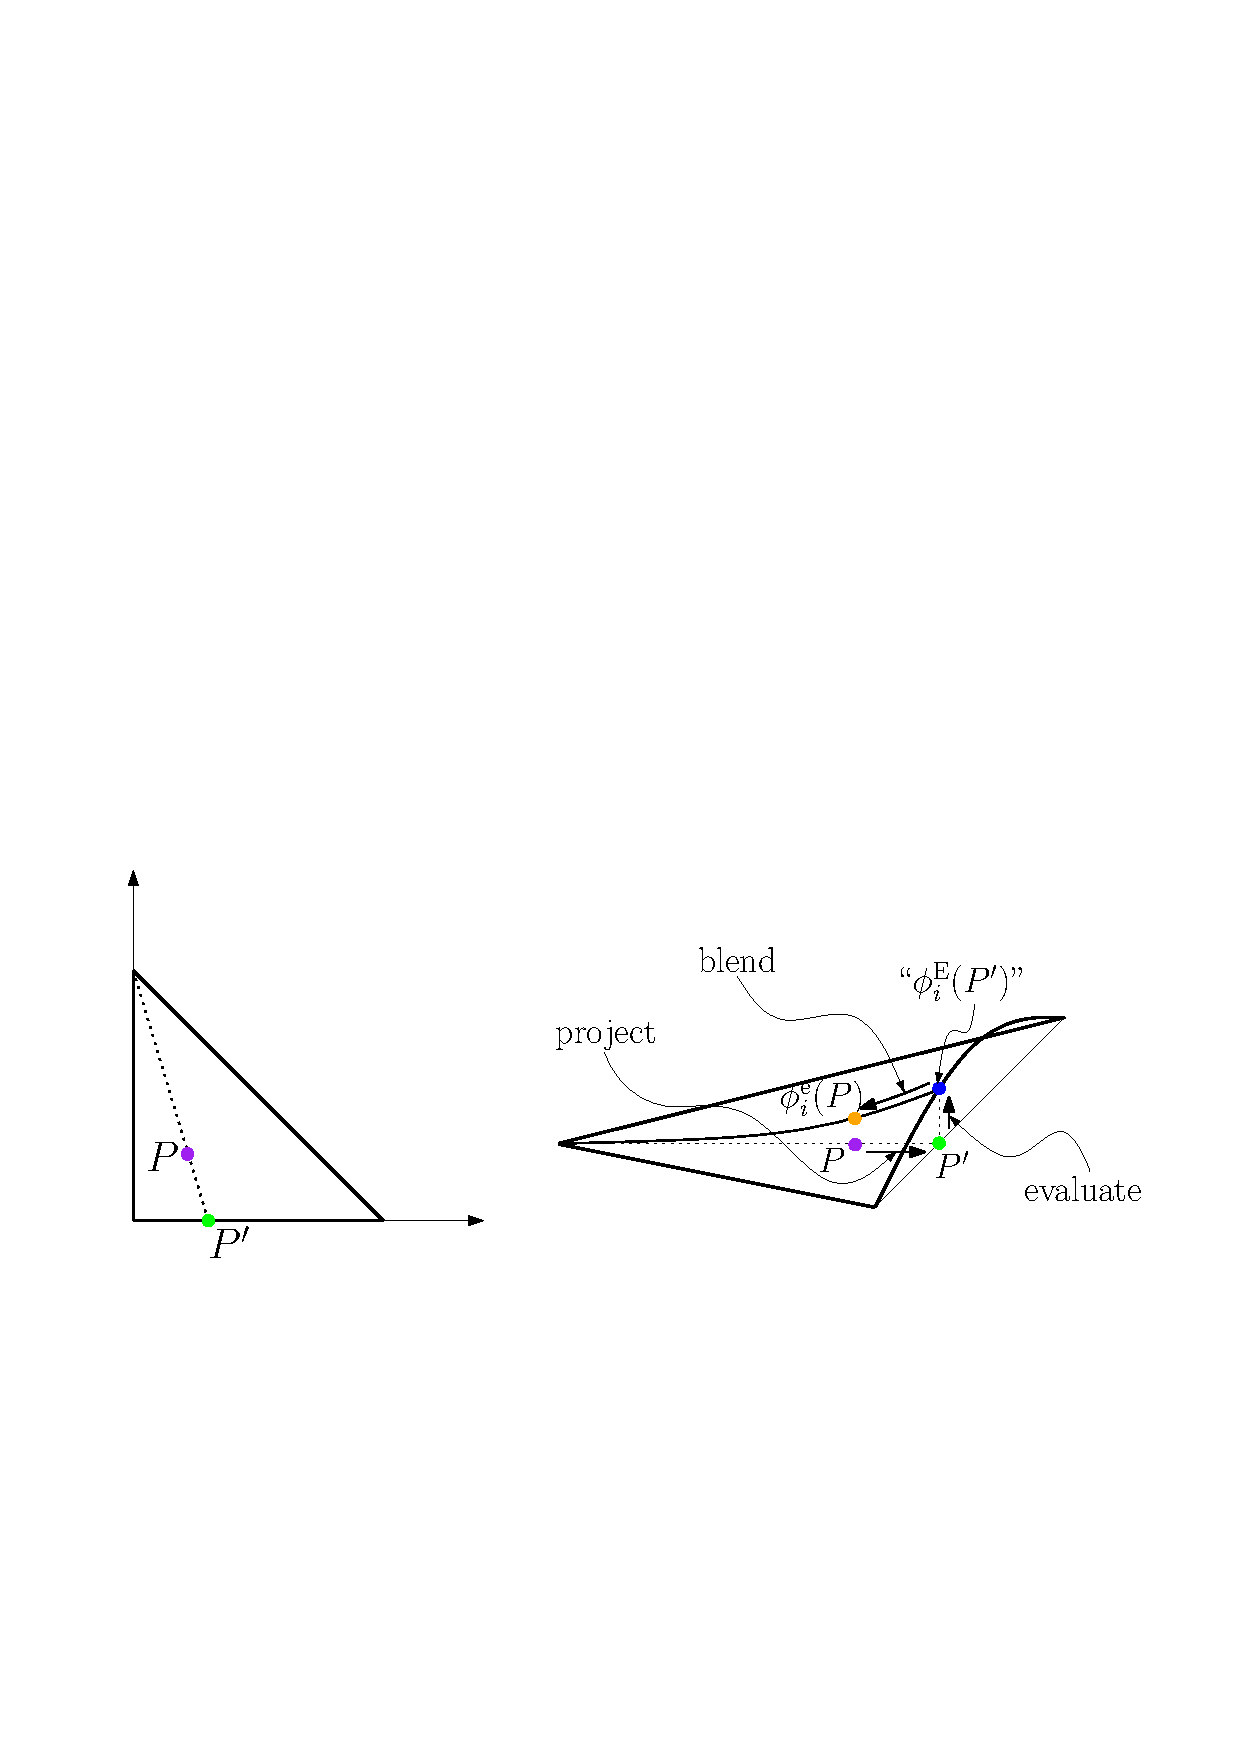
\includegraphics[scale=0.55]{./figures/TriangleProjection.pdf}
\caption{Edge projection from $P$ to $P'$, and the logic project$\,\to\,$evaluate$\,\to\,$blend.}
\label{fig:TriangleProjection}
\end{center}
\end{figure}

As with the quadrilateral, there is a geometrical interpretation to these expressions, and again it follows the fundamental logic of project$\,\to\,$evaluate$\,\to\,$blend, which is marked below:
\begin{equation*}
    \phi_i^\mathrm{e}(x)=\phi_i^\E(\vec{\nu}_{01}(x))
    	=\underbrace{(\nu_0(x)+\nu_1(x))^i}_{\text{blend}}
    		\underbrace{\phi_i^\E\Big(\underbrace{\textstyle{\frac{\nu_0(x)}{\nu_0(x)+\nu_1(x)}},
    			\textstyle{\frac{\nu_1(x)}{\nu_0(x)+\nu_1(x)}}}_{\text{project}}\Big)}_{\text{evaluate}}\,.
    				%=(\nu_0(x)+\nu_1(x))^i
    				%	[L_i]\Big(\textstyle{\frac{\nu_0(x)}{\nu_0(x)+\nu_1(x)}},\textstyle{\frac{\nu_1(x)}{\nu_0(x)+\nu_1(x)}}\Big)\,,
\end{equation*}
The coordinates $(\frac{\nu_0}{\nu_0+\nu_1},\frac{\nu_1}{\nu_0+\nu_1})$ are projected 1D coordinates, because they sum to $1$ for all $x$. 
Note this is \textit{not} true for the coordinates $(\nu_0,\nu_1)$ in general (only over the edge itself).
As argued before for the quadrilateral, the projected coordinates represent a point over edge 01:
\begin{equation*}
	(x_1,x_2)\;\longmapsto\;(\textstyle{\frac{x_1}{1-x_2}},0)\,.
\end{equation*}
Geometrically, it consists of finding the intersection $P'=(\frac{x_1}{1-x_2},0)$ of the edge with the projecting line passing through the original point $P=(x_1,x_2)$ and the disjoint opposite vertex. 
This projection and the logic of the construction is illustrated in Figure \ref{fig:TriangleProjection}.

%Note that in this case, the blending function is hiding within the homogenization process, and it is a \textit{nonlinear} function. Also, notice $\tilde{\mu}_1=\frac{\nu_1}{\nu_0+\nu_1}\in[0,1]$, since $\nu_1\geq0$ and $\nu_0\geq0$ by the properties of affine coordinates. Indeed, $\tilde{\mu}_1$ represents a projected coordinate. More explicitly, the two dimensional projection to edge 01 is
%\begin{equation*}
%	(x_1,x_2)\;\longmapsto\;(\textstyle{\frac{x_1}{1-x_2}},0)\,.
%\end{equation*}
%It consists of finding the intersection $P'=(\frac{x_1}{1-x_2},0)$ of the edge with the projecting line passing through the original point $P=(x_1,x_2)$ and the opposite vertex to the edge. This is illustrated in Figure \textit{add Figure}. Finally it is easy to check the desired trace properties:
%\begin{alignat*}{4}
%	&[L_i](\nu_0(x),\nu_1(x))|_{x_2=0}&&=[L_i](\mu_0(x_1),\mu_1(x_1))&&=L_i(x_1)\\
%	&[L_i](\nu_0(x),\nu_1(x))|_{x_2=1-x_1}&&=[L_i](0,x_1)&&=0\\
%	&[L_i](\nu_0(x),\nu_1(x))|_{x_1=0}&&=[L_i](1-x_1-x_2,0)&&=0\,.
%\end{alignat*}

%It should now be clear why $\phi_i^\E$ was defined so generally before in (\textit{put reference}). 
The complete list of edge functions with their gradients is
\begin{equation}
	\phi_i^\mathrm{e}(x)=\phi_i^\E(\vec{\nu}_{ab}(x))\,,\qquad\quad\nabla\phi_i^\mathrm{e}(x)=\nabla\phi_i^\E(\vec{\nu}_{ab}(x))\,,
	\label{eq:Triphigeneral}
\end{equation}
with $i=2,\ldots,p$, and $0\leq a<b\leq2$ (so $(a,b)=(0,1),(1,2),(0,2)$). As usual, there are a total of $p-1$ edge functions for every edge, for a total of $3(p-1)$ edge functions.
%
%\paragraph{Edge Orientations}
%To consider orientations, first look at the predefined local edge axis for a given edge, and replace $\phi_i^\E$ by $\phi_i^{\e,\oo}$ with the appropriate entries. 
%The oriented edge functions, which have supercript $\e,\oo$, are explained in \S\ref{sec:edgeorientations}.
%For example, take edge 01. 
%The predefined local edge axis $\xi^\mathrm{e}$ for this edge points from vertex 0 to vertex 1.
%This means the order of the entries in $\phi_i^{\e,\oo}$ is $(\nu_0(x),\nu_1(x))$ (and $\textit{not}$ $(\nu_1(x),\nu_0(x))$ which would apply if the local edge axis pointed from vertex 1 to vertex 0).
%This defines the $\oo=0$ orientation.
%Hence, for edge 12, \eqref{eq:Triphigeneral} becomes
%\begin{equation*}
%    \phi_i^\mathrm{e}(x)=\phi_i^{\e,\oo}(\nu_0(x),\nu_1(x))
%        =\begin{cases}
%            \phi_i^{\e,0}(\nu_0(x),\nu_1(x))
%            	=\phi_i^{\e}(\nu_0(x),\nu_1(x))\,\,\,&\text{if }\oo=0\\
%            \phi_i^{\e,1}(\nu_0(x),\nu_1(x))
%            	=\phi_i^{\e}(\nu_1(x),\nu_0(x))\,\,\,&\text{if }\oo=1\,,
%        \end{cases}
%\end{equation*}
%where \eqref{eq:orientEdge} was used as the definition of $\phi_i^{\e,\oo}$. The same applies to the gradients, and the other edge functions that follow in $H(\mathrm{curl})$ (which involve $E_i^\E$).
%

%We begin with a reintroduction of a construction of the 1D edge bubbles using affine coordinates. Let $p\geq2$ be the order of the edge and let $\hat\phi_i(t), t \in [0,1]$, be a polynomial of order $2\leq i\leq p$, vanishing at $t = 0,1$. Our default choice will be the shifted Lobatto polynomial,
%\be
%\hat\phi_i(t) = L_i(t) = L_i(t; 1) \, .
%\ee
%Introducing the affine edge coordinates:
%\be
%\mu_0 = 1 - t,\quad \mu_1 = t \, ,
%\ee
%we can represent function $\hat\phi_i$ in the form:
%\be
%\hat\phi_i(t) = \phi_i (\mu_0,\mu_1)
%\ee
%where function $\phi_i$ is a polynomial of (total) degree $i$
%in terms of the edge affine coordinates $\mu_0,\mu_1$. Given local affine coordinates $s_0,s_1$ of the $0-1$ edge (the construction is independent of the spatial dimension), we define the unoriented affine edge shape functions as:
%\be
%\phi^\E_i(s_0,s_1) = [\phi_i] (s_0,s_1) = \phi_i\left(\frac{s_0}{s_0+s_1},
%\frac{s_1}{s_0+s_1}\right) (s_0 + s_1)^i \, , \quad i=2,\ldots,p
%\label{eq:EdgeShap2}
%\ee
%where $p$ is the edge order.
%The map prescribing for a point in the triangle
%the corresponding point on the edge with edge coordinates:
%\be
%\mu_n = \frac{s_n}{s_0+s_1},\quad n=0,1\, ,
%\ee
%can be viewed as a projection onto the edge, whereas function
%$(s_0 + s_1)^i$ is the edge blending function.
%
%\begin{figure}[ht!]
%    \centering
%    \begin{subfigure}[b]{0.45\textwidth}
%        \includegraphics[width=\textwidth]{./figures/tri_V2.png}
%        \caption{Edge $H^1$ bubble for the triangle.}
%        \label{fig:H1edgebub_tri}
%    \end{subfigure}%
%\end{figure}
%    ~ %add desired spacing between images, e. g. ~, \quad, \qquad, \hfill etc.
%      %(or a blank line to force the subfigure onto a new line)
%    %\begin{subfigure}[b]{0.45\textwidth}
%    %    \includegraphics[width=\textwidth]{./tet_V2.png}
%    %    \caption{Edge $H^1$ bubble projection for the tet.}
%    %    \label{fig:H1edgebub_tet}
%    %\end{subfigure}
%    %\caption{Edge shape functions.}\label{fig:H1edgebub_tet}
%% \label{fig:H1bub_tri}
%%\end{figure}
%
%Contrary to the square or hexahedral element, the first term on the right hand side of Equation~\eqref{eq:EdgeShap2} {\em is not} a polynomial, however, the product {\em is}.
%As we will be using integrated polynomials $\left[L_i\right](\nu_1,\nu_0) = \phi^{\e}_i(\nu_0,\nu_1)$ we have that \begin{equation}\phi^{\e}_i(\nu_0,\nu_1)= \left[L_i\right](\nu_1,\nu_0) = L_i(\nu_0;\nu_0+\nu_1) \nonumber \end{equation}
%
%
%Moreover, it is not difficult to see that the edge shape function $\phi^\E_i(\nu_0,\nu_1)$ satisfies the required vanishing property. Indeed, by construction, $\phi^\E_i(\nu_0,\nu_1)$ is nonzero on the $0-1$ edge and zero on the other two edges. Also, $\nabla \phi^\E_i(\nu_0,\nu_1)$ lies in the proper N\'ed\'elec space.


%\paragraph{Orientation Considerations} We now consider the case where we have oriented edges, which, as we saw in the 1D case, was obtained by a simple permutation of the order of arguments in the shape function. In the triangle case, the situation is similar. Indeed, if we wish to consider the oriented case with orientation $\oo=1$, we {\em define} $\phi^{\e,\oo}_i(\nu_0,\nu_1) = \left[L_i\right](\nu_1,\nu_0) = L_i(\nu_0;\nu_0+\nu_1)$.
%With the above definition, we find that the set of $H^1$ edge shape functions on the $0-1$ edge for the triangle are given as
%\be
%\phi^{\e,\oo}_i(\nu_0,\nu_1) =
%\left\{
%    \begin{array}{ll}
%        \phi_i^{E}(\nu_0,\nu_1) = L_i(\nu_1;\nu_0+\nu_1) & \text{if } \oo = 0\\
%        \phi_i^{E}(\nu_1,\nu_0) = L_i(\nu_0;\nu_0+\nu_1) & \text{if } \oo = 1
%    \end{array}
%\right.
%\ee
%
%The full family of all edge shape functions for the triangle (and line segment) is composed of the shape functions above, $\phi^\E_i$, considered on each edge independently.
%% For simplicity, we have assumed unswapped coordinates in each case above.
%
%% We leave it as a simple excercise for the reader to show that if we allow for $i=1$ in the definiton~\eqref{eq:H1_CountingSimplexEdge}, then $\phi_1(s_k,s_l)$ agrees with the vertex shape functions defined previously, albeit with some overcounting in the case of the tetrahedron.
%% \textcolor{red}{Provide pictorial illustration of the projection in
%% both 2D and 3D.}
%
%
%% \textcolor{red}{Provide a pictorial example in 2D for an edge shape function}

\subsubsection{\texorpdfstring{$H^1$}{H1} Face Bubbles}

These intuitively involve all three affine coordinates $(\nu_0,\nu_1,\nu_2)$.% as opposed to only two of them (like the edges).
The first natural idea is to use the existing edge shape functions and multiply by another function $\hat{\phi}_j$ which vanishes at the remaining edge.
That is,
\begin{equation*}
	\phi_{ij}^\mathrm{f}(x)=\phi^\E_i(\nu_0(x),\nu_1(x))\hat{\phi}_j(\nu_2(x))\,.
\end{equation*}
Here, $\hat{\phi}_j(y)$ should also be an $H^1$ function with domain $y\in[0,1]$ (since $0\leq\nu_2(x)\leq1$) and which vanishes at $y=0$, so that $\hat{\phi}_j(0)=0$. 
Notice that in the quadrilateral, when constructing $\phi_{ij}^\Box$ the choice was naturally $\hat{\phi}_j=L_j$ since it was required that $\hat{\phi}_j(0)=\hat{\phi}_j(1)=0$, so it should vanish at \textit{both} endpoints. 
%Moreover, that case extends the pattern naturally to the hexahedron. 
For the triangle there is much more liberty for the choice of $\hat{\phi}_j$, and indeed it can be chosen such that it has many advantages. 
Following \citet{Beuchler_Schoeberl_06} it is chosen as a Jacobi polynomial, $\hat{\phi}_j=L_j^\alpha$, with $\alpha=2i$, where $i$ is the order of $\phi^\E_i$. This results in
\begin{equation*}
	\phi_{ij}^\mathrm{f}(x)=\phi^\E_i(\nu_0(x),\nu_1(x))L_j^{2i}(\nu_2(x))\,.
\end{equation*}

Thinking ahead to the tetrahedron, this definition can be easily generalized. Just as with $\phi_i^\E$, the generalization is nothing more than the homogenization of the previous formula, as written in \eqref{eq:homogproduct}.%As with edge to triangle, extension to tetrahedron, so more general definition next.

\begin{definition*}
Let $s_0$, $s_1$ and $s_2$ be arbitrary functions of some spatial variable in $\R^N$, with $N=2,3$, and denote by $p_s$ the order in the coordinate triplet $(s_0,s_1,s_2)$. Then
\begin{equation}
    \phi_{ij}^\Tri(s_0,s_1,s_2)=\phi_i^\E(s_0,s_1)[L_j^{2i}](s_0+s_1,s_2)=[L_i,L_j^{2i}](s_0,s_1,s_2)\,,
\end{equation}
for $i\geq2$, $j\geq1$ and $n=i+j=3,\ldots,p_s$. %$($or equivalently $i=n-j$, $j=1,\ldots,n-2$ and $n=i+j=3,\ldots,p$$)$. 
The gradients, understood in $\R^N$, are
\begin{equation}
    \begin{aligned}
    \nabla\phi_{ij}^\Tri(s_0,s_1,s_2)&=[L_j^{2i}](s_0+s_1,s_2)\nabla\phi_i^\E(s_0,s_1)
    	+\phi_i^\E(s_0,s_1)\nabla[L_j^{2i}](s_0+s_1,s_2)\,,
    \end{aligned}
\end{equation}
where for any $\alpha$,
\begin{equation}	
	\begin{aligned}
  	\nabla[L_j^\alpha](s_0\!+\!s_1,s_2)&=[P_{j-1}^\alpha](s_0\!+\!s_1,s_2)\nabla s_2
  		+[R_{j-1}^\alpha](s_0\!+\!s_1,s_2)\nabla(s_0\!+\!s_1\!+\!s_2)\\
        &=P_{j-1}^\alpha(s_2;s_0\!+\!s_1\!+\!s_2)\nabla s_2
        		+R_{j-1}^\alpha(s_2;s_0\!+\!s_1\!+\!s_2)\nabla(s_0\!+\!s_1\!+\!s_2)\,.
  \end{aligned}\label{eq:DerivativeofLalpha}
\end{equation}
\end{definition*}

% \be
% \phi^\f_{ij} = \phi^\E_i \left(\frac{\nu_0}{\nu_0+\nu_1},\frac{\nu_1}{\nu_0+\nu_1}\right)
% (\nu_0 + \nu_1)^i \, \hat\phi_j (\nu_2)
% \ee
%\be
%\phi^\Tri_{ij}(\nu_0,\nu_1,\nu_2) = \phi^\E_i \left(\nu_0,\nu_1\right) \hat\phi_j (\nu_2)
%\ee
%with
%$$
%i\ge2,\, j\ge1,\, i+j \leq p
%$$
%where $p$ is the order of the triangle and $\hat{\phi}_j(t),\,  t \in [0,1]$, is a polynomial of order $j$ vanishing at $t=0$.
%% Here $\phi^\E_i$ is an affine representation of a 1D $H^1$ bubble of order $i$, and polynomial $\hat{\phi}_j(x),\,  x \in [0,1]$, vanishes at $x=0$.
% Following Sven Beuchler and Joachim Sch\"{o}berl \textit{cite},
%we define \mbox{$\hat\phi_j := L^{2i-1}_{j}$}, the integrated shifted Jacobi polynomial with weight $\alpha = 2i-1$ and order $j$. In this case, we arrive at
%\be
%\begin{array}{ll}
%\phi^\Tri_{ij}(\nu_0,\nu_1,\nu_2) & = L_i(\frac{\nu_1}{\nu_0 + \nu_1}) (\nu_0 + \nu_1)^i L^{2i-1}_{j}(\nu_2)
%\\[8pt]
%& = L_i(\nu_1; \nu_0 + \nu_1) L^{2i-1}_{j}(\nu_2)
%\\[8pt]
%& = \left[L_i,L^{2i-1}_{j}\right](\nu_0,\nu_1,\nu_2)
%\end{array}
%\label{eq:H1_TriFace}
%\ee
%where in the final line we have used the property $\nu_0+\nu_1+\nu_2=1.$

%Again, we note that the vanishing property is satisfied by construction. The edge function $\phi^\E_i \left(\nu_0,\nu_1\right)$ vanishes on all edges except the $0-1$ edge, while the $H^1$ bubble $\hat\phi_j (\nu_2)$ vanishes when $\nu_2=0$, i.e., on the $0-1$ edge, so that the product, $\phi^\Tri_{ij}(\nu_0,\nu_1,\nu_2)$ vanishes on the entire boundary of the triangle, and is non-zero in the interior. Moreover, by a calculation entirely analogous to the edge case, the gradients of the face functions also lie in the appropriate space.
Note the indexing was shown as $i\geq2$, $j\geq1$ and $n=i+j=3,\ldots,p_s$. 
In many $hp$ codes it is useful to enforce hierarchy, so that the shape functions are organized by total order. 
That is, first list all order $3$ bubbles, then all order $4$ bubbles, and so on.
Hence when coding is in mind, it is useful to have an outer loop with numbering $n=3,\ldots,p_s$ and an inner loop indexing with either $i=2,\ldots,n-1$ (so $j=n-i$) or $j=1,\ldots,n-2$ (so $i=n-j$).

Regarding the vanishing properties of this new ancillary function, it suffices to rewrite \eqref{eq:LiLjvanishing} so that for any $s_0,s_1,s_2$, and all $i\geq2$, $j\geq1$,
\begin{equation}
	\phi_{ij}^\Tri(s_0,s_1,0)=\phi_{ij}^\Tri(s_0,0,s_2)=\phi_{ij}^\Tri(0,s_1,s_2)=0\,.\label{eq:phiTrivanishing}
\end{equation}

As expected, when the coordinates are 2D affine coordinates, the formulas for $\phi_{ij}^\Tri$ and its gradient are simplified.
For this, record the next remark.

\begin{remark}
Let $\nu_0=1-\nu_1-\nu_2$, where $\nu_1$ and $\nu_2$ are arbitrary functions of some spatial variable in $\R^N$, $N=2,3$, and where $p$ is the order in the coordinates $(\nu_0,\nu_1,\nu_2)$. Then for all $i\geq2$, $j\geq1$, and $n=i+j=3,\ldots,p$,
\begin{equation}
	\begin{aligned}
    \phi_{ij}^\Tri(\nu_0,\nu_1,\nu_2)&=\phi_i^\E(\nu_0,\nu_1)L_j^{2i}(\nu_2)\,,\\
    \nabla\phi_{ij}^\Tri(\nu_0,\nu_1,\nu_2)&=L_j^{2i}(\nu_2)\nabla\phi_i^\E(\nu_0,\nu_1)
    	+\phi_i^\E(\nu_0,\nu_1)P_{j}^{2i}(\nu_2)\nabla\nu_2\,.
	\end{aligned}
  \label{eq:H1Trispecialcase}
\end{equation}
\end{remark}


%Note the numbering was quoted as $i=n-j$, $j=1,\ldots,n-2$ and $n=3,\ldots,p$, which translates to $i\geq2$, $j\geq1$ and $n=i+j=3,\ldots,p$. The reason for this numbering is to enforce the idea that the triangle functions should be organized by total order. Hence, in a code the outer loop is in $n$, then $j$ and finally $i=n-j$ is fixed dependent on $n$ and $j$.  That is,
%\begin{verbatim}
%do n=3,...,p
%    do j=2,...,n-2
%        i=n-j
%        ...
%    enddo
%enddo
%\end{verbatim}
%Ensuring this hierarchy in total order is useful in many $hp$ codes.

%Also, observe that in two dimensions, where $\nu_0+\nu_1+\nu_2=1$, the formula collapses to the one proposed initially, while the formula for the gradients simplifies to
%\begin{align*}
%	\phi_{ij}^\Tri(\nu_0,\nu_1,\nu_2)&=L_j^{2i-1}(\nu_2)\nabla\phi_i^\E(\nu_0,\nu_1)
%		+\phi_i^\E(\nu_0,\nu_1)(P_{j-1}^{2i-1}(\nu_2;1)\nabla\nu_2+R_{j-1}^{2i-1}(\nu_2;1)\nabla1)\\
%			&=L_j^{2i-1}(\nu_2)\nabla\phi_i^\E(\nu_0,\nu_1)+\phi_i^\E(\nu_0,\nu_1)P_{j-1}^{2i-1}(\nu_2)\nabla\nu_2\,.
%\end{align*}

%The full family of all $H^1$ triangle face bubbles are simply the functions above, $\phi^\Tri
%_{ij}$. In this case orientations are not important and we need only construct one set of shape functions from blending a single family of edge shape functions (in this case, $\nu_2=0$);
%As usual, it is preferred to write all formulas in terms of $\phi_{ij}^\Tri$. This will be useful when orientations are introduced. 
In general, the $H^1$ triangle face bubbles and their gradients are
\begin{equation}
	\phi_{ij}^\mathrm{f}(x)=\phi_{ij}^\Tri(\vec{\nu}_{012}(x))\,,\qquad\quad
		\nabla\phi_{ij}^\mathrm{f}(x)=\nabla\phi_{ij}^\Tri(\vec{\nu}_{012}(x))\,,
% \phi^\f_{ij}(\nu_0,\nu_1,\nu_2)% = \left[L_i\right](s_k,s_l)
\label{eq:H1_CountingTriFace}
\end{equation}
where $i\geq2$, $j\geq1$ and $n=i+j=3,\ldots,p$. 
The vanishing conditions are satisfied by construction or simply by looking at \eqref{eq:phiTrivanishing}. 
There are a total of $\frac{1}{2}(p-1)(p-2)$ $H^1$ face bubbles for the triangle.

% \be
% \left\{\phi(x)\in\mathcal{P}^p(\hat\Delta) : \phi(x) = \phi^\f_{ij}(\nu_0(x),\nu_1(x),\nu_2(x))
% % \phi^\f_{ij}(\nu_0,\nu_1,\nu_2)% = \left[L_i\right](s_k,s_l)
%  \, , \quad i\ge2,\, j\ge1,\, i+j\leq p\right\}\,.
% \label{eq:H1_CountingTriFace}
% \ee

%\begin{remark}
%When coding, in order to enforce the hierarchy in the order of the shape functions, here and afterwards for other shape functions on simplices, construct a loop iterating in total order of the polynomial space. For example
%\begin{verbatim}
%do k=3,...,p
%    do j=1,...,p-2
%        i=k-j
%        ...
%    end
%end
%\end{verbatim}
%\end{remark}


%\paragraph{\texorpdfstring{$H^1$}{H1} Linear Independence}
%
%To account for all of the constructed shape functions for the triangle, we set $d=2$ and sum all of the shape functions constructed in Equations~\eqref{eq:H1_CountingSimplexVert}, \eqref{eq:H1_CountingSimplexEdge}, and \eqref{eq:H1_CountingTriFace}:
%\be
%3+3(p-1)+{p-1\choose 2} = {p+2\choose 2}
%\ee
%which is equal to the dimension of $\mathcal{P}^p$ for $d=2$.
%The linear independence of the above shape functions, using the presented Lobatto and integrated Jacobi polynomials is given for the triangle in \textit{cite Beuchler} and \textit{cite}.
%
%Since the cardinality of our set of linearly independent shape functions agrees with the dimension of $\mathcal{P}^p$ for both the triangle, we understand that our set is spanning and that we have constructed an appropriate basis for the space.

\subsection{\texorpdfstring{$H(\mathrm{curl})$}{Hcurl} Shape Functions}

%As a reminder, in two dimensions, the trace of $H(\mathrm{curl})$ functions is the tangential component of the vector function along the boundary (that is, the edges).
%Hence, all edge functions should have vanishing trace at all other edges, while the bubbles should have zero trace at all edges. 

The dimension of $\mathcal{N}^p$ in two dimensions is $p(p+2)$.
A careful count of the linearly independent conforming shape functions to be presented throughout this section will coincide with that dimension. 
Showing that the functions constructed are in $\mathcal{N}^p$ is nontrivial, but will follow from the next instrumental lemma.% where one must recall the definition of $H(\mathrm{curl})$ edge functions in \eqref{eq:Hcurledgefunctions}.

\begin{lemma}
\label{lemma:curl}
Let $x\in\R^N$ for $N=2,3$, and $f_n\in\mathcal{P}^n(x)$ be any polynomial of total order $n$ in the coordinates $x=(x_1,\ldots,x_N)$. Given $s_0$ and $s_1$ coordinates in $\mathcal{P}^1(x)$ $($linear functions in $x$$)$, it follows that the N\'ed\'elec space of order $n+1$, $\mathcal{N}^{n+1}$, contains the function
\begin{equation*}
	f_n(\bcdot)\Big(s_0\nabla s_1-s_1\nabla s_0\Big)\in\mathcal{N}^{n+1}\,.
\end{equation*}
\end{lemma}
\begin{proof}
Recall the definition of the N\'ed\'elec space,
\begin{equation*}
	\mathcal{N}^p=(\mathcal{P}^{p-1})^N\oplus\Big\{E\in(\tilde{\mathcal{P}}^{p})^N: x\cdot E(x)=0\,\text{ for all } 
		x\in\R^N\Big\}\,.
\end{equation*}
The (affine) coordinates are linear functions in $x=(x_1,\ldots,x_N)$, so that
\begin{equation*}
	s_k(x)=a_k+b_k\cdot x\,,
\end{equation*}
for $a_k\in\R$, $b_k\in\R^N$ and $k=0,1$. As a result $\nabla s_k(x)=b_k$, and
\begin{equation*}
	s_0(x)\nabla s_1(x)-s_1(x)\nabla s_0(x)=\underbrace{(a_0b_1-a_1b_0)}_{=A}+\underbrace{((b_0\cdot x)b_1-(b_1\cdot x)b_0)}_{=B(x)}\,.
\end{equation*}
Clearly, $A\in(\mathcal{P}^0)^N=\R^N$, while $B\in(\tilde{\mathcal{P}}^1)^N$. Moreover,
\begin{equation*}
	x\cdot B(x)=x\cdot((b_0\cdot x)b_1-(b_1\cdot x)b_0)=(b_0\cdot x)(b_1\cdot x)-(b_1\cdot x)(b_0\cdot x)=0\,,
\end{equation*}
so that $B\in\{E\in(\tilde{\mathcal{P}}^{1})^N: x\cdot E(x)=0\}$, and $s_0\nabla s_1-s_1\nabla s_0\in\mathcal{N}^1$.

Now, $f_n\in\mathcal{P}^n=\mathcal{P}^{n-1}\oplus\tilde{\mathcal{P}}^n$, for $n\geq1$ can always be decoupled into $f_n=f_{n-1}+\tilde{f}_n$, where $f_{n-1}\in\mathcal{P}^{n-1}$ and $\tilde{f}_n\in\tilde{\mathcal{P}}^n$. As a result
\begin{equation*}
	f_n(x)(s_0(x)\nabla s_1(x)-s_1(x)\nabla s_0(x))=f_n(x)A+f_{n-1}(x)B(x)+\tilde{f}_n(x)B(x)\,,
\end{equation*}
where it is clear $f_{n}A+f_{n-1}B\in(\mathcal{P}^n)^N$ and $\tilde{f}_nB\in(\tilde{\mathcal{P}}^{n+1})^N$. Meanwhile, 
\begin{equation*}
x\cdot(\tilde{f}_n(x)B(x))=\tilde{f}_n(x)x\cdot B(x)=0\,.
\end{equation*}
Hence, $f_n(\bcdot)(s_0\nabla s_1-s_1\nabla s_0)\in\mathcal{N}^{n+1}$.
\end{proof}



%\begin{proof}\,
%We begin with the observation that the homogenization operation
%\be
%[\cdot]:\mathcal{P}^n\to\tilde{\mathcal{P}^n}
%\ee
%is surjective. In this case, any monomial in $f_n\in\tilde{\mathcal{P}^n}$ may be expressed as
%\be
%f_n(s_0,s_1) = g_n\left(\frac{s_0}{s_0+s_1},\frac{s_1}{s_0+s_1}\right)\left(s_0+s_1\right)^n,
%\ee
%for some $g_n\in\mathcal{P}^n$. We now see, by direct computation, that
%\begin{align*}
%\bfnab\times E(s_0,s_1) &= \bfnab\times \left(f_n(s_0,s_1) [s_0 \bfnab s_1 - s_1 \bfnab s_0 ]\right)\\
%&= \bfnab \left(g_n\left(\frac{s_0}{s_0+s_1},\frac{s_1}{s_0+s_1}\right)\left(s_0+s_1\right)^n\right) \times [s_0 \bfnab s_1 - s_1 \bfnab s_0 ] + f_n(s_0,s_1) \bfnab\times [s_0 \bfnab s_1 - s_1 \bfnab s_0 ]\\
%&= \bfnab g_n\left(\frac{s_0}{s_0+s_1},\frac{s_1}{s_0+s_1}\right)\left(s_0+s_1\right)^n \times [s_0 \bfnab s_1 - s_1 \bfnab s_0 ]\\
%&\quad + g_n\left(\frac{s_0}{s_0+s_1},\frac{s_1}{s_0+s_1}\right) n \left(s_0+s_1\right)^{n-1}\left(\bfnab s_0 + \bfnab s_1\right) \times [s_0 \bfnab s_1 - s_1 \bfnab s_0 ] \\
%&\quad + 2f_n(s_0,s_1) \bfnab s_0 \times \bfnab  s_1\\
%&= (n+2) \, f_n(s_0,s_1) \, \bfnab s_0 \times \bfnab  s_1 \, ,
%\end{align*}
%since
%\be
%\bfnab g_n\left(\frac{s_0}{s_0+s_1},\frac{s_1}{s_0+s_1}\right) \quad \parallel \quad [s_0 \bfnab s_1 - s_1 \bfnab s_0 ] \, .
%\ee
%
%Now, let $x = (x_1,\ldots,x_N)\in\hat\Delta$ be the Cartesian coordinates of $x$. Then,
%\be
%s_k = a_k + \sum_{i=1}^Nb_{ki}x_i,
%\ee
%where $a_k,b_{ki}\in\mathbb{R}$, $k=1,2$, $i=1,\ldots,N$. Since each $s_k$ is an affine function, $s_0 \bfnab s_1 - s_1 \bfnab s_0 \in \left(\mathcal{P}^{1}\right)^d$. Moreover, letting $\{\bfe_i\}_{i=1}^N$ be the Euclidean basis,
%\be
%s_0 \bfnab s_1 - s_1 \bfnab s_0 = \sum_{i=1}^N\left(a_0 b_{1i}-a_1 b_{0i}\right)\bfe_i + \sum_{i,j=1}^N\left( b_{0i}b_{1j}-b_{1i}b_{0j}\right)x_i\bfe_j,
%\ee
%where
%\be
%%a_0\sum_{i=1}^N b_{1i}\bfe_i-a_1\sum_{i=1}^N b_{0i}\bfe_i
%\sum_{i=1}^N\left(a_0 b_{1i}-a_1 b_{0i}\right)\bfe_i \in \left(\mathcal{P}^0\right)^d,
%\ee
%and
%\be
%%\left(\sum_{i=1}^N b_{0i}x_i\right)\left(\sum_{i=1}^N b_{1i}\bfe_i\right)-\left(\sum_{i=1}^N b_{1i}x_i\right)\left(\sum_{i=1}^N b_{0i}\bfe_i\right)
%\sum_{i,j=1}^N\left( b_{0i}b_{1j}-b_{1i}b_{0j}\right)x_i\bfe_j \in \left(\tilde{\mathcal{P}}^1\right)^d.
%\ee
%Moreover,
%\be
% x \cdot \sum_{i,j=1}^N\left( b_{0i}b_{1j}-b_{1i}b_{0j}\right)x_i\bfe_j = \sum_{i,j=1}^N\left( b_{0i}b_{1j}-b_{1i}b_{0j}\right)x_ix_j = 0.
%\ee
%Therefore,
%\be
%s_0 \bfnab s_1 - s_1 \bfnab s_0 \in \mathcal{N}^1,
%\ee
%and the general result follows.
%
%\end{proof}

\subsubsection{\texorpdfstring{$H(\mathrm{curl})$}{Hcurl} Edges}

Having seen what ocurred with $H^1$ edge functions due to the process of homogenization, it is wise to consider the general definition of $H(\mathrm{curl})$ edge functions in \eqref{eq:Hcurledgefunctions}, using 2D affine coordinates as entries. 
Indeed this will suffice.
For instance, for edge 01, the shape functions are
\begin{equation*}
	\begin{aligned}
		E_i^\mathrm{e}(x)&=E_i^\E(\vec{\nu}_{01}(x))=[P_i](\vec{\nu}_{01}(x))\Big(\nu_0(x)\nabla\nu_1(x)-\nu_1(x)\nabla\nu_0(x)\Big)\\
    	&=(\nu_0(x)+\nu_1(x))^i
    		[P_i]\Big(\textstyle{\frac{\nu_0(x)}{\nu_0(x)+\nu_1(x)}},\textstyle{\frac{\nu_1(x)}{\nu_0(x)+\nu_1(x)}}\Big)
    			E_0^\E(\vec{\nu}_{01}(x))\\
    	&=\underbrace{(\nu_0(x)+\nu_1(x))^{i+2}}_{\text{blend}}
    		\underbrace{E_i^\E\Big(\underbrace{\textstyle{\frac{\nu_0(x)}{\nu_0(x)+\nu_1(x)}},
    			\textstyle{\frac{\nu_1(x)}{\nu_0(x)+\nu_1(x)}}}_{\text{project}}\Big)}_{\text{evaluate}}\,,
	\end{aligned}
\end{equation*}
for $i=0,\ldots,p-1$. 
By Lemma \ref{lemma:curl} it easily follows $E_i^\mathrm{e}\in\mathcal{N}^{i+1}\subseteq\mathcal{N}^{p}$ as desired.
The tangential trace properties are also satisfied. 
To see this, it suffices to look at $E_0^\mathrm{e}$, since $E_i^\mathrm{e}(x)=[P_i](\vec{\nu}_{01}(x))E_0^\mathrm{e}(x)$. 
Its traces are
\begin{alignat*}{3}
    &\mathrm{tr}(E_0^\mathrm{e}(x))|_{x_2=0}&&=E_0^\E(\vec{\nu}_{01}(x))|_{\nu_2=0}\cdot(v_1-v_0)
    	=\nabla\nu_1(x)\cdot(v_1-v_0)=1\,,\\
    &\mathrm{tr}(E_0^\mathrm{e}(x))|_{1-x_1-x_2=0}&&=E_0^\E(\vec{\nu}_{01}(x))|_{\nu_0=0}\cdot(v_2-v_1)
    	=-\nu_1(x)\nabla\nu_0(x)\cdot(v_2-v_1)=0\,,\\
  	&\mathrm{tr}(E_0^\mathrm{e}(x))|_{x_1=0}&&=E_0^\E(\vec{\nu}_{01}(x))|_{\nu_1=0}\cdot(v_2-v_0)
  		=\nu_0(x)\nabla\nu_1(x)\cdot(v_2-v_0)=0\,.
\end{alignat*}
Here the vanishing traces follow from the fact that the gradient of a function is always perpendicular to the tangents of its isosurfaces. 
Hence $\nabla\nu_0(x)$ is perpendicular to the tangents of the set where $\nu_0(x)=0$, which is precisely where $v_2-v_1$ lies. 
Regarding the nonzero trace, the formula $\nabla\nu_1(x)\cdot(v_1-v_0)$ follows after replacing $\nu_0=1-\nu_1$, and noting that $\nabla(\nu_0(x)+\nu_1(x))\cdot(v_1-v_0)=-\nabla\nu_2(x)\cdot(v_1-v_0)=0$.

More generally, the edge functions and their curls are
\begin{equation}
	E_i^\mathrm{e}(x)=E_i^\E(\vec{\nu}_{ab}(x))\,,\qquad\quad\nabla\times E_i^\mathrm{e}(x)=\nabla\times E_i^\E(\vec{\nu}_{ab}(x))\,,
	\label{eq:TriEgeneral}
\end{equation}
with $i=0,\ldots,p-1$, and $0\leq a<b\leq2$ (so $(a,b)=(0,1),(1,2),(0,2)$). There are a total of $p$ edge functions for every given edge, giving a total of $3p$ edge functions.
%It can also be readily checked that the desired trace properties are satisfied. 
%That is, the (tangential) trace is of the form $P_{i}(x_a)$ for some $a=1,2$ over edge $ab$ and zero over the other two edges.
%Moreover, by Lemma \ref{lemma:curl} it easily follows $E_i^\mathrm{e}\in\mathcal{N}^{i+1}$ for all $i=0,\ldots,p-1$.





%Consider the $0-1$ edge of the triangle and let $p$ be the order of this edge. In unlike the $H^1$ case, in $H(\text{curl})$ we no longer need an endpoint vanishing property for the edge shape functions. % Ultimately, the shape of shape functions restricted to a given edge should conform to $??(\marhbb{R})$ instead of $H^{1/2}(\mathbb{R})$.
%Given the have a larger space of polynomials available to us (one without endpoint conditions), we describe a new notation: let $\hat\psi_i\in\mathcal{P}^{p-1}$ be any given polynomial of order $i\leq p-1$.
%
%Without taking into account embedded orienations, for an edge with endpoint affine coordinates $\nu_0,\nu_1$, we define the affine $H(\text{curl})$ edge functions by:
%\be
%E^\E_i(\nu_0,\nu_1) = \left[\hat\psi_i\right](\nu_0,\nu_1)
%(\nu_0 \bfnab \nu_1 - \nu_1 \bfnab \nu_0 )\, , \quad i=0,\ldots,p-1\,.
%\label{eq:edge_curl}
%\nonumber
%\ee
%If $\hat\psi_i = P_i$, where $P_i$ denotes the shifted scaled Legendre polynomial of order $i$, then clearly, $$\left[\hat\psi_i\right] = \left[P_i\right]\,,$$
%\be
%E^{e}_i(x_1,x_2)= E^\E_i(\nu_0,\nu_1) = \left[P_i\right](\nu_0,\nu_1)
%(\nu_0 \bfnab \nu_1 - \nu_1 \bfnab \nu_0 )\, , \quad i=0,\ldots,p-1\,.
%\label{eq:edge_curl_1}
%\nonumber
%\ee
%and by Lemma~\ref{lemma:curl},
%\be
%\bfnab \times E_i^\E(\nu_0,\nu_1) =  (i+2) \, \left[P_i\right](\nu_0,\nu_1) \,
%\bfnab \nu_0 \times \bfnab \nu_1 \, .
%\nonumber
%\ee
%Note that for $i=0$ we obtain the Whitney edge functions and all functions live in the Ned\'{e}l\'{e}c space of ``order'' $i + \half$,
%\be
%E^\mathrm{e}_i \in \mathcal{N}^i\,.
%\ee
%Note also that in general, we have the following formula for the edge shape functions:
%
%\be
%E^{e}_i(x_1,x_2) = E^\E_i(\nu_a,\nu_b) = \left[P_i\right](\nu_a,\nu_b)
%(\nu_a \bfnab \nu_b - \nu_b \bfnab \nu_a )\, , \quad i=0,\ldots,p-1\,,
%\label{eq:edge_curl_2}
%\nonumber
%\ee
%where $a,b = 0,1,2$ and $a\leq b$
%\paragraph{Orientation Consideration}
%
%Taking into account orientation changes on the edge, as before we have the following orientation embedded definitons for the affine $H(\text{curl})$ edge functions
%\be
%E^{\e,\oo}_i(\nu_0,\nu_1) =
%\left\{
%    \begin{array}{ll}
%        \left[P_i\right](\nu_0,\nu_1)\left(\nu_0 \bfnab \nu_1 - \nu_1 \bfnab \nu_0\right) & \text{if } \oo =0 \\
%        \left[P_i\right](\nu_1,\nu_0)\left(\nu_1 \bfnab \nu_0 - \nu_0 \bfnab \nu_1\right) & \text{if } \oo =1
%    \end{array}
%\right.
%\ee
%for the triangle.

\subsubsection{\texorpdfstring{$H(\mathrm{curl})$}{Hcurl} Face Bubbles}

The construction of $H(\mathrm{curl})$ face bubbles is parallel to that of $H^1$ bubbles. 
The idea is to multiply $H(\mathrm{curl})$ edge functions with an $H^1$ function vanishing at zero. 
%Again, there is some liberty in the choice of the $H^1$ function. 
Again, it is chosen according to \citet{Beuchler_Pillwein_Zaglmayr_13} as the Jacobi polynomial, $L_j^\alpha$, with $\alpha=2i+1$, where $i$ is the order of $E^\E_i$.
Like the quadrilateral, the triangle has two closely related families generated by the same ancillary operator defined below.
%In fact there are two closely related families.
%They are defined generally below.

\begin{definition*}
Let $s_0$, $s_1$ and $s_2$ be arbitrary functions of some spatial variable in $\R^N$, with $N=2,3$, and denote by $p_s$ the order in the coordinate triplet $(s_0,s_1,s_2)$. Then
\begin{equation}
    E_{ij}^\Tri(s_0,s_1,s_2)=[L_j^{2i+1}](s_0+s_1,s_2)E_i^\E(s_0,s_1)\,,
\end{equation}
for $i\geq0$, $j\geq1$ and $n=i+j=1,\ldots,p_s-1$.
%$i=n-j$, $j=1,\ldots,n$ and $n=1,\ldots,p-1$ $($or equivalently $i\geq0$, $j\geq1$ and $n=i+j=1,\ldots,p-1$$)$. 
The curls, understood in $\R^N$, are
\begin{equation}
    \begin{aligned}
    \nabla\!\times\! E_{ij}^\Tri(s_0,s_1,s_2)&\!=\![L_j^{2i+1}](s_0\!+\!s_1,s_2)\nabla\!\times\! E_i^\E(s_0,s_1)
    	\!+\!\nabla[L_j^{2i+1}](s_0\!+\!s_1,s_2)\!\times\! E_i^\E(s_0,s_1)\,,
    \end{aligned}
\end{equation}
where $\nabla[L_j^{2i+1}](s_0+s_1,s_2)$ is computed from \eqref{eq:DerivativeofLalpha}.
%Also,
%\begin{equation}
%    \begin{aligned}
%    E_{ij}^{\Delta_{II}}(s_0,s_1,s_2)&=E_{ij}^{\Delta_{I}}(s_1,s_2,s_0)\,,\qquad\quad
%    	\nabla\times E_{ij}^{\Delta_{II}}(s_0,s_1,s_2)=\nabla\times E_{ij}^{\Delta_{I}}(s_1,s_2,s_0)\,,
%    \end{aligned}
%\end{equation}
%for $i=n-j$, $j=1,\ldots,n$ and $n=1,\ldots,p-1$ $($or equivalently $i\geq0$, $j\geq1$ and $n=i+j=1,\ldots,p-1$$)$.
\end{definition*}

As with the edge functions, it is clear that when evaluated in any permutation of $(\nu_0,\nu_1,\nu_2)$ the vanishing trace properties are satisfied.
The two families defined below give a total of $p(p-1)$ $H(\mathrm{curl})$ triangle face bubbles (each family has $\frac{1}{2}p(p-1)$).
%In view of this, each family has $\frac{1}{2}p(p-1)$, so that there is a total of $p(p-1)$ $H(\mathrm{curl})$ triangle face bubbles. 
%In both families the vanishing properties are satisifed by construction.

\subparagraph{Family I:} 
The shape functions for the first family and their curl are
\begin{equation}
	E_{ij}^{\mathrm{f}}(x)=E_{ij}^\Tri(\vec{\nu}_{012}(x))\,,\qquad\quad
		\nabla\times E_{ij}^{\mathrm{f}}(x)=\nabla\times E_{ij}^\Tri(\vec{\nu}_{012}(x))\,,
\end{equation}
for $i\geq0$, $j\geq1$ and $n=i+j=1,\ldots,p-1$. 
By Lemma \ref{lemma:curl}, $E_{ij}^\mathrm{f}\in\mathcal{N}^{n+1}$, where $n=i+j$. 
There are $\frac{1}{2}p(p-1)$ bubble functions in this family.
%The vanishing properties can be readily checked. There are $\frac{1}{2}p(p-1)$ $H(\mathrm{curl})$ face bubbles in this family.

\subparagraph{Family II:}
The shape functions for the second family and their curl are
\begin{equation}
	E_{ij}^{\mathrm{f}}(x)=E_{ij}^\Tri(\vec{\nu}_{120}(x))\,,\qquad\quad
		\nabla\times E_{ij}^{\mathrm{f}}(x)=\nabla\times E_{ij}^\Tri(\vec{\nu}_{120}(x))\,,
\end{equation}
for $i\geq0$, $j\geq1$ and $n=i+j=1,\ldots,p-1$.
The only difference with the first family is that the entries are permuted to $\vec{\nu}_{120}(x)=(\nu_1(x),\nu_2(x),\nu_0(x))$ instead of $\vec{\nu}_{012}(x)=(\nu_0(x),\nu_1(x),\nu_2(x))$.
Again, they lie in $E_{ij}^\mathrm{f}\in\mathcal{N}^{n+1}$, where $n=i+j$, and there are $\frac{1}{2}p(p-1)$ bubble functions in this family.

%Let $p$ be the order of the triangle face and
%$$i \geq 0,\, j \geq 1,\quad i+j=1,\ldots,p-1\,.$$
%
%Continuing the logic of the construction of affine $H^1$ triangle bubbles and edge $H(\text{curl})$ functions, we define the {\em first family} of triangle $H(\text{curl})$ bubbles as follows:
%\be
%E^\mathrm{f}_{ij}(x) = E^\Tri_{ij}(\nu_0(x),\nu_1(x),\nu_2(x))\,,
%\ee
%where
%\begin{align}
%E^\Tri_{ij}(\nu_0,\nu_1,\nu_2) &= E^\E_{i}(\nu_0,\nu_1) \, L^{2i-1}_{j}(\nu_2)
%\nonumber\\
%& = \left[P_i,L^{2i-1}_{j}\right](\nu_0,\nu_1,\nu_2)(\nu_0 \bfnab \nu_1 - \nu_1 \bfnab \nu_0 )\, .
%\label{eq:Hcurl_Face1}
%\end{align}
%In the above equation we recall that $E^\E_{i}$ is the $H(\text{curl})$ edge shape function corresponding to the first triangle edge, see (), and $L^{2i-1}_{j}$ denotes the shifted integrated Jacobi polynomial with weight $2i-1$ and order $j$.
%%\ref{eq:edge_curl}
%This motivates the the following definition for a generic function. Given arguments $s_0,s_1,s_2$ of a simplex (triangle, tetrahedron), we define the following two sets of {$H(\text{curl})$} triangle bubbles.
%
%\begin{definition*} Given the bubble function $E^\Tri_{ij}(s_0(x),s_1(x),s_2(x))$ with arguments $s_0(x),s_1(x),s_2(x)$, the corresponding two sets of $H(\text{curl})$ triangle bubbles are: \\$E^{\Delta_I}_{ij}(s_0(x),s_1(x),s_2(x)) = E^\Tri_{ij}(s_0(x),s_1(x),s_2(x)) \\
%E^{\Delta_II}_{ij}(s_0(x),s_1(x),s_2(x)) = E^\Tri_{ij}(s_1(x),s_2(x),s_0(x))$ \\
%where $E^\Tri_{ij}(s_0(x),s_1(x),s_2(x)) =  \left[P_i,L^{2i-1}_{j}\right](s_0(x),s_1(x),s_2(x))(s_0 \bfnab s_1 - s_1 \bfnab s_0 )$
%\\\end{definition*}

% Above,
% $$
% \bfnab L^{2i-1}_{j}(\nu_2) = \frac{d L^{2i-1}_{j}}{dx} (\nu_2)
% \, \bfnab \nu_2 = P^{2i-1}_{j-1} (\nu_2)
% \, \bfnab \nu_2\, .
% $$
%The above definition, as applied to the case of affine coordinates yields two sets of triangle bubbles, one set of triangle bubbles is constructed by rotating the indices of the other\footnote{Only one rotation of the indices is required to span this space}.

%\begin{description}
%  \item[Family I:]
%\be
%E^\mathrm{f}_{ij}(x) = E^\Tri_{ij}(\nu_0(x),\nu_1(x),\nu_2(x)),\quad i \geq 0,\, j \geq 1,\quad i+j=1,\ldots,p-1
%\ee
%
%  \item[Family II:]
%\be
%E^\mathrm{f}_{ij}(x) = E^\Tri_{ij}(\nu_1(x),\nu_2(x),\nu_0(x)),\quad i \geq 0,\, j \geq 1,\quad i+j=1,\ldots,p-1\,.
%\ee
%
%\end{description}


%\paragraph{\boldmath{$H(\text{curl})$} Linear Independence}
%
%Note that for the triangle, we have
%\be
%3p+2{p\choose 2} = p(p+2)
%\ee
%shape functions.


\subsection{\texorpdfstring{$H(\mathrm{div})$}{Hdiv} Shape Functions}
\label{sec:TriangleHdiv}

In two dimensions, the $H(\mathrm{div})$ space (see \eqref{eq:Hdiv2Ddef}) is isomorphic to $H(\mathrm{curl})$. 
%Indeed, this is achieved simply by rotating the $H(\mathrm{curl})$ functions. 
Indeed, just like with the quadrilateral, given a shape function $E\in H(\mathrm{curl})$ and its curl $\nabla\times E\in L^2$, the corresponding $H(\mathrm{div})$ shape function with its divergence is
\begin{equation}
    V=\begin{pmatrix}0&1\\-1&0\end{pmatrix}E\,,\quad\qquad\nabla\cdot V=\nabla\times E\,.
\end{equation}
Although not immediate, note that in \textit{two} dimensions the original polynomial space $\mathcal{N}^p$ for $H(\mathrm{curl})$ simply becomes the $H(\mathrm{div})$ conforming space $\mathcal{RT}^p$ after the rotation, as required.


\subsection{\texorpdfstring{$L^2$}{L2} Shape Functions}

These span $\mathcal{P}^{p-1}$, so there should be $\frac{1}{2}p(p+1)$ linearly independent shape functions.

\subsubsection{\texorpdfstring{$L^2$}{L2} Face}

%Analagous to the construction of the $H^1$ triangle bubbles, we use homogenization to construct the $L^2$-conforming shape functions for the triangle. In this case, the arguments have no special continuity properties for traces, and we define
Again, carefully chosen Jacobi polynomials are present in this construction. 
%The former ensures that the shape functions lie in $\mathcal{P}^{p-1}$, as required.
The shape functions are
\begin{equation}
\begin{aligned}
	\psi_{ij}^\mathrm{f}(x)&=[P_i](\nu_0(x),\nu_1(x))[P_j^{2i+1}](\nu_0(x)+\nu_1(x),\nu_2(x))\\
		&=[P_i,P_j^{2i+1}](\vec{\nu}_{012}(x))(\nabla\nu_1(x)\!\!\times\!\!\nabla\nu_2(x))\,,
\end{aligned}
\end{equation}
where $i\geq0$, $j\geq0$ and $n=i+j=0,\ldots,p-1$.
%$i=n-j$, $j=0,\ldots,n$ and $n=0,\ldots,p-1$ (or equivalently $i\geq0$, $j\geq0$ and $n=i+j=0,\ldots,p-1$). 
Clearly the functions lie in $\mathcal{P}^{p-1}$ and there are $\frac{1}{2}p(p+1)$ such functions. 
The factor $\nabla\nu_1(x)\!\times\!\nabla\nu_2(x)$ makes the expression coordinate free (with the $x$ coordinates it is $1$).
%$$
%i,j \geq 0,\quad i+j=0,\ldots,p-1 \, .
%$$

%\paragraph{\texorpdfstring{$L^2$}{L2} Linear Independence}
%
%In this final space, we clearly have
%\be
%{p+1\choose2}
%\ee
%shape functions for the triangle.
%
%The verification that we have constructed a basis follows similarly from the $H^1$ case.

\subsection{Orientations}
\label{sec:TriaOrientations}

Only edge orientations are required to ensure compatibility of 2D triangles.
However, in 3D elements, triangle \textit{faces} have the notion of orientation, and one needs to consider this to ensure full compatibility.
In \S\ref{sec:QuadEdgeOrientations} it was shown how to apply the principles introduced in \S\ref{sec:edgeorientations} to construct orientation embedded edge functions.
It is convenient to have read those sections.
In what follows, a brief illustration of how it analogously applies to the triangle is given in \S\ref{sec:TriaEdgeOrientations}.
Afterwards, in \S\ref{sec:TriaFaceOrientations}, the triangle face orientations are described.

\subsubsection{Edge Orientations}
\label{sec:TriaEdgeOrientations}

\begin{figure}[!ht]
\begin{center}
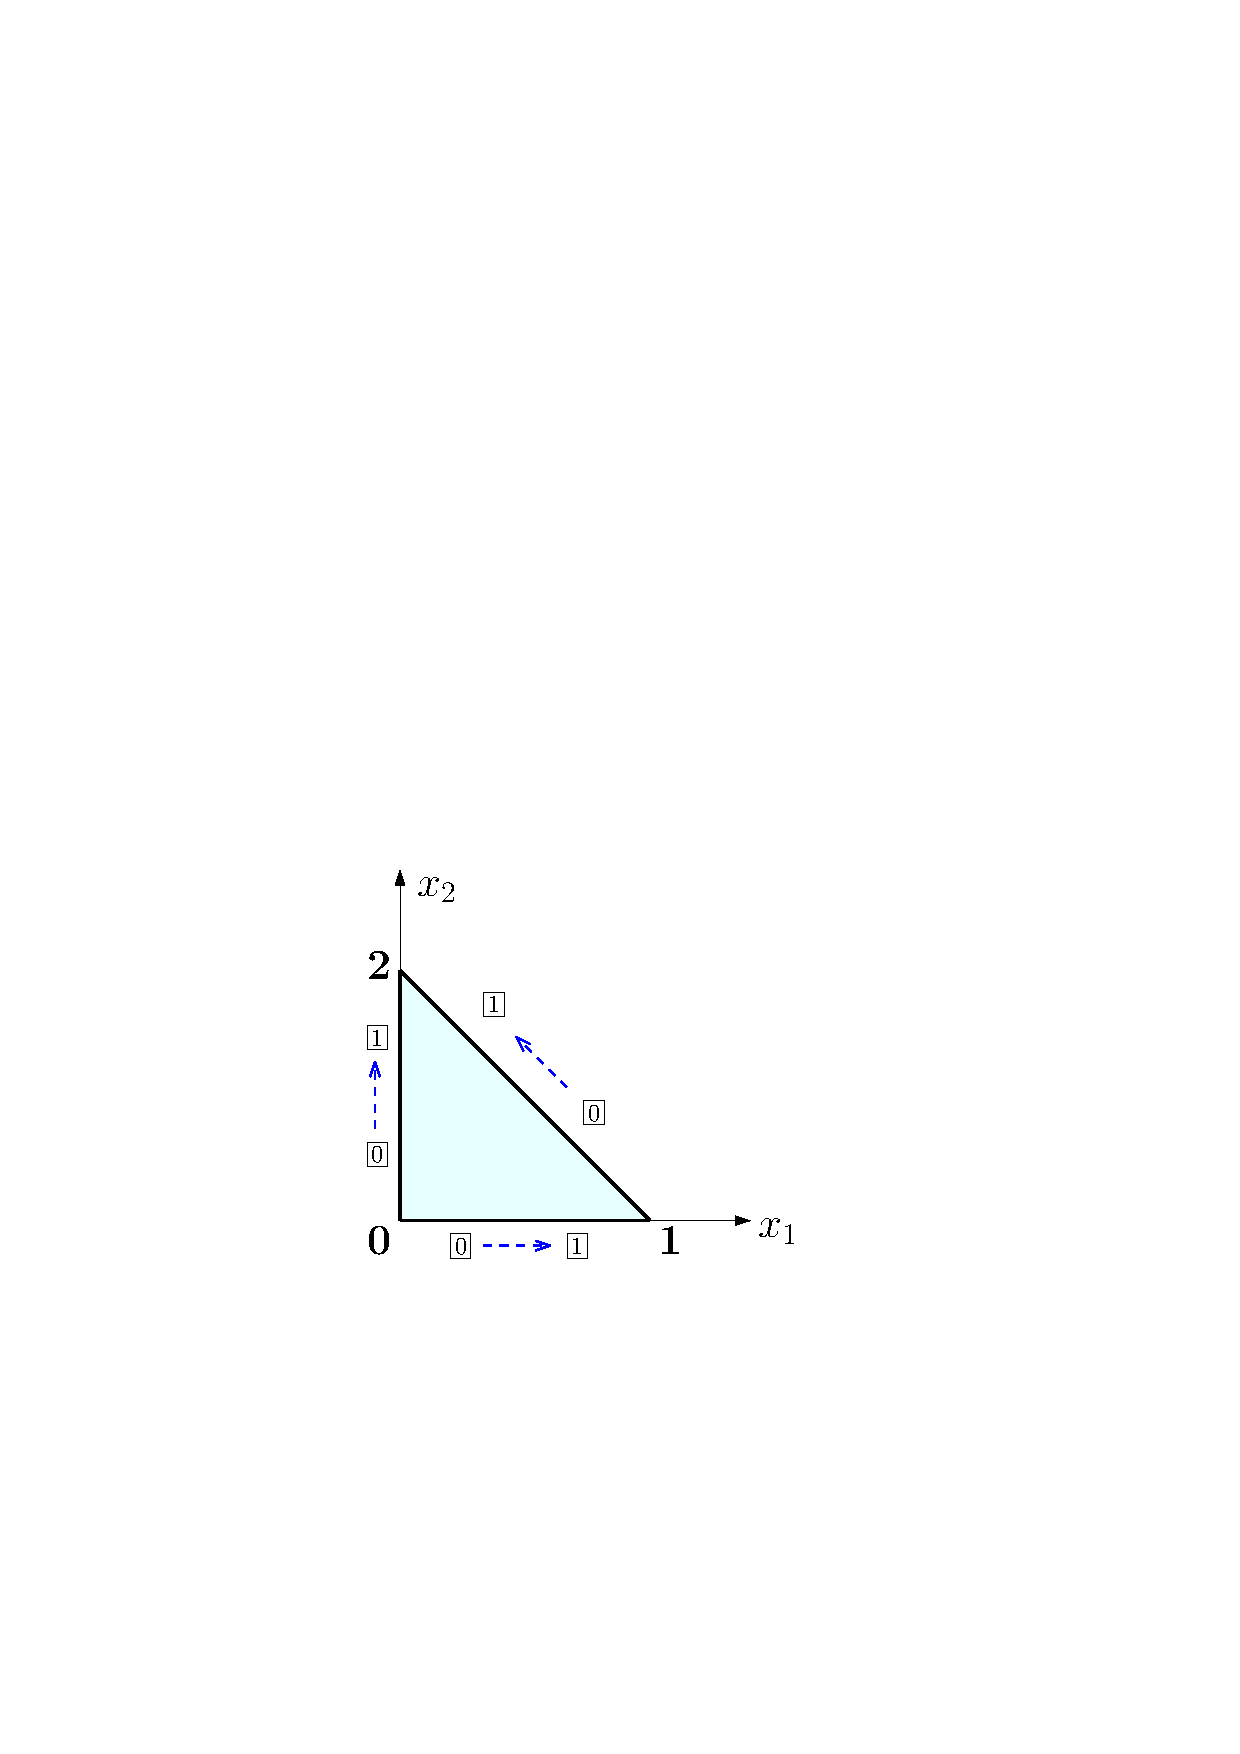
\includegraphics[scale=0.5]{./figures/MasterTriOrientations.pdf}
\caption{Master triangle with local edge orientations.}
\label{fig:MasterTriOrientations}
\end{center}
\end{figure}

The master triangle has a predefined \textit{local} orientation for each edge, which reperesents the $\oo=0$ case. 
These are shown in Figure \ref{fig:MasterTriOrientations}.
They are \textit{our} choices for the local orientations.

As with the quadrilateral, the local orientations induce a master element \textit{local} edge vertex-ordering which then determines a \textit{locally ordered} pair of affine coordinates. 
In the triangle, the correspondence between vertices and affine coordinates is trivial, since all one needs to know is that the vertex $v_a$ is linked to the affine coordinate $\nu_a$, where $a=0,1,2$.
As an example take the local edge orientations shown in Figure \ref{fig:MasterTriOrientations}.
Then, it is clear that the induced \textit{local} edge vertex-orderings are $v_0\tdashto v_1$, $v_1\tdashto v_2$ and $v_0\tdashto v_2$ for edges 01, 12 and 02 respectively.
Therefore, the \textit{locally ordered} pair of coordinates are $(\nu_0,\nu_1)$, $(\nu_1,\nu_2)$ and $(\nu_0,\nu_2)$.
These are then transformed to a \textit{globally ordered} pair via the edge local-to-global transformation $\sigma_\oo^\E$, and inputted into the different ancillary functions to give the orientation embedded shape functions.
For example, for edge 01, the orientation embedded $H^1$ edge functions are
\begin{equation*}
    \phi_i^\mathrm{e}(x)=\phi_i^\E\circ\sigma_\oo^\E(\vec{\nu}_{01}(x))
        =\begin{cases}
            \phi_i^\E\Big(\sigma_0^\E(\vec{\nu}_{01}(x))\Big)
            	=\phi_i^\E(\vec{\nu}_{01}(x))\,\,\,\text{if }\oo=0\,,\\
            \phi_i^\E\Big(\sigma_1^\E(\vec{\nu}_{01}(x))\Big)
            	=\phi_i^{\e}(\vec{\nu}_{10}(x))\,\,\,\text{if }\oo=1\,,
        \end{cases}
\end{equation*}
for $i=2,\ldots,p$.
For a more detailed example which analogously applies to the triangle see \S\ref{sec:QuadEdgeOrientations}.

\subsubsection{Triangle Face Orientations Explained}
\label{sec:TriaFaceOrientations}

%With triangles (as with quadrilaterals) it is not important to consider face orientations, since the boundary, which is shared with adjacent elements, is one dimensional.
%This means only edge orientations need to be considered.
%However, in three dimensions, the boundary is two dimensional and triangle faces will be shared by adjacent elements.
%It is required to match the corresponding shape functions over these faces to satisfy the compatibility condition.

In 3D, each face at the mesh must be given its own \textit{global face orientation} to ensure full compatibility across the boundaries.
For triangles, this is represented by the global triangle face coordinates $\Xi^\Tri=(\Xi_1^\Tri,\Xi_2^\Tri)$, or equivalently, by the \textit{global face vertex-ordering}.
For instance, given a triangle face in the mesh, a vertex-ordering of the form $a\tto b\tto c$ means the origin of $\Xi^\Tri$ is located at $a$, $\Xi_1^\Tri$ points from $a$ to $b$, and $\Xi_2^\Tri$ points from $a$ to $c$.
Meanwhile, at the master element, the mapped face has its own fixed \textit{local orientation}.
It is represented by the coordinates $\xi^\Tri=(\xi_1^\Tri,\xi_2^\Tri)$ or equivalently by the fixed \textit{local} ordering of the form $\boxednum{0}\!\tdashto\boxednum{1}\!\tdashto\boxednum{2}$.
In general, the two systems of coordinates will not match, and this mismatch is represented by the orientation parameter $\oo$.
For triangle faces, there are \textit{six} possible orientations, meaning $\oo=0,\ldots,5$.
These are all illustrated in Figure \ref{fig:OrientationsTri}.

\begin{figure}[!ht]
\begin{center}
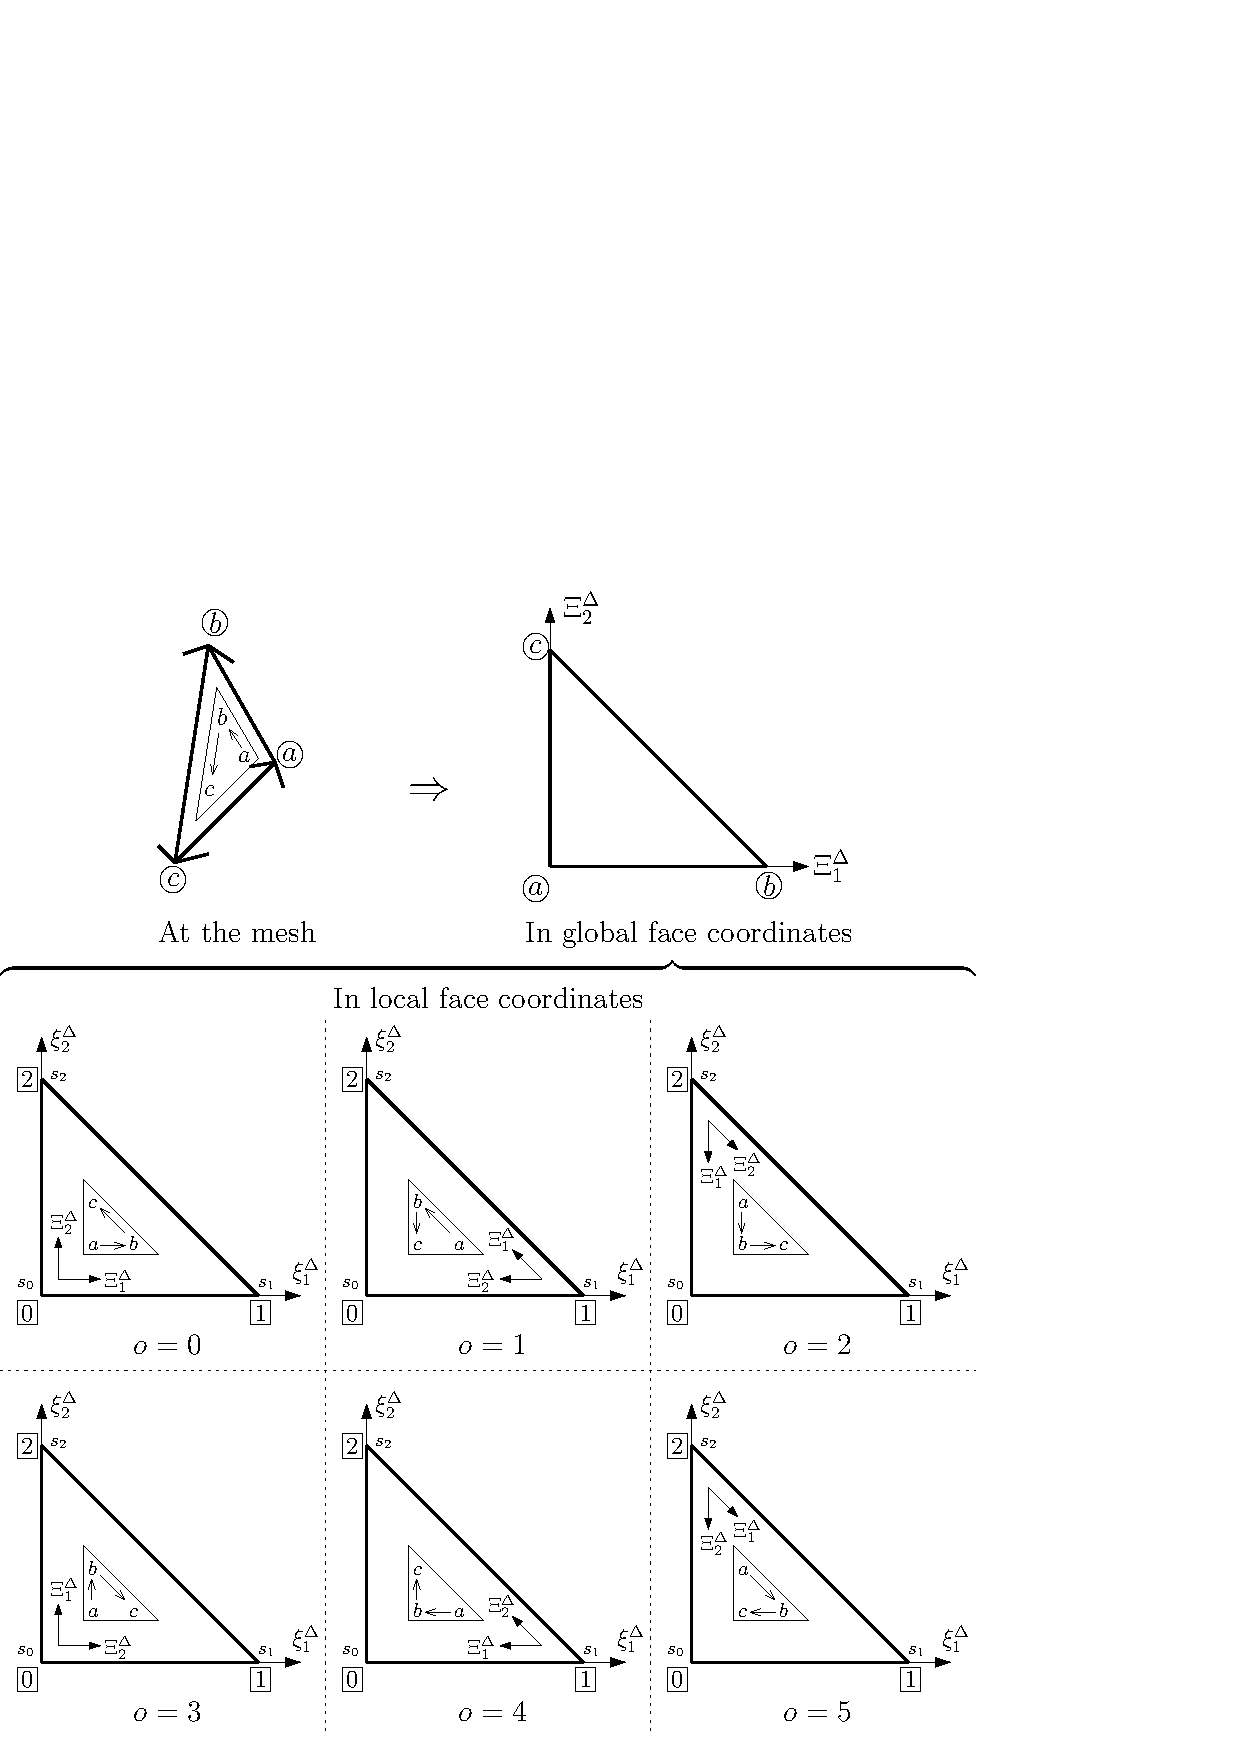
\includegraphics[scale=0.75]{./figures/OrientationsTriangle.pdf}
\caption{Triangle face orientations.}
\label{fig:OrientationsTri}
\end{center}
\end{figure}

Like quadrilaterals and edges, one needs a local-to-global transformation dependent on $\oo$.
For this, the \textit{local} orientation is represented by the \textit{locally ordered} triplet $(s_0,s_1,s_2)$.
The \textit{global} orientation is analogously represented by a \textit{globally ordered} triplet naturally induced from the \textit{global face vertex-ordering}.
For example, looking at Figure \ref{fig:OrientationsTri}, when $\oo=1$, the global ordering $a\tto b\tto c$ corresponds to the ordering $\boxednum{1}\!\tto\boxednum{2}\!\tto\boxednum{0}$, which in turn coresponds to the globally ordered triplet $(s_1,s_2,s_0)$.
Hence, once again the local-to-global transformation can be represented by a permutation, $\sigma_\oo^\Tri$, dependent on $\oo$.
It can be determined by observing Figure \ref{fig:OrientationsTri}.
Subsequently, all that is required is to compose the \textit{triangle face} ancillary functions and their differential form (those with superscript $\Tri$) with the local-to-global transformation $\sigma_\oo^\Tri$.
This should be done in all 3D shape functions associated to triangle faces.
More concrete examples will be given later.
Finally, the permutation function, $\sigma_\oo^\Tri$, is precisely defined next.

\begin{definition*}
Let $s_0$, $s_1$ and $s_2$ be arbitrary variables, and let $\oo=0,1,2,3,4,5$ be the triangle face orientation parameter. 
The triangle face orientation permutation function, $\sigma_\oo^\Tri$, is defined as
\begin{equation}
	\sigma_\oo^\Tri(s_0,s_1,s_2)=\begin{cases}
		\sigma_0^\Tri(s_0,s_1,s_2)=(s_0,s_1,s_2)&\quad\text{if  }\,\oo=0\,,\\
		\sigma_1^\Tri(s_0,s_1,s_2)=(s_1,s_2,s_0)&\quad\text{if  }\,\oo=1\,,\\
		\sigma_2^\Tri(s_0,s_1,s_2)=(s_2,s_0,s_1)&\quad\text{if  }\,\oo=2\,,\\
		\sigma_3^\Tri(s_0,s_1,s_2)=(s_0,s_2,s_1)&\quad\text{if  }\,\oo=3\,,\\
		\sigma_4^\Tri(s_0,s_1,s_2)=(s_1,s_0,s_2)&\quad\text{if  }\,\oo=4\,,\\
		\sigma_5^\Tri(s_0,s_1,s_2)=(s_2,s_1,s_0)&\quad\text{if  }\,\oo=5\,.\end{cases}\label{eq:orientTriFace}
\end{equation}
\end{definition*}

%In the case of triangles, everything can be understood by the way the three triangle vertices are listed. 
%For every face there is a predefined local numbering of the vertices, symbolized by $\xi^\mathrm{f}$ while there is a global numbering of the vertices, symbolized by $\Xi^\mathrm{f}$. There are \textit{six} different ways in which the vertices can be numbered. 
%That is, \textit{six} different possible global orientations represented by the parameter $\oo=0,\ldots,5$. They are shown in Figure \textit{add Figure}.
%
%Fortunately, these orientations are handled simply by permuting the entries of the triangular face functions: $\phi_{ij}^\Tri$, $E_{ij}^{\Delta_I}$, $E_{ij}^{\Delta_{II}}$, and in the future $V_{ij}^\Tri$.
%However, it should be mentioned that nontrivial pullback transforms are ocurring internally (but automatically) in the functions when the entries are permuted.
%
%To explain these permutations, the function $\vec{\sigma}$ is introduced as
%\begin{equation}
%    \begin{alignedat}{2}
%        \vec{\sigma}:\{0,1,2,3,4,5\}&\,\longrightarrow\,\{0,1,2\}\times\{0,1,2\}\times\{0,1,2\}\\
%        \oo\,&\,\longmapsto\,(\sigma_1(\oo),\sigma_2(\oo),\sigma_3(\oo))\,.
%    \end{alignedat}
%\end{equation}
%The function is more explicitly specified in Table \ref{table:functionSigma}.
%
%\begin{table}[ht]
%\begin{center}
%\begin{tabular}
%{|c|c|c|c|}\hline
%$\oo$ &$\sigma_1(\oo)$ & $\sigma_2(\oo)$  &  $\sigma_3(\oo)$ \\\hline\hline
%0 &0 & 1  & 2 \\\hline
%1 &2 & 0  & 1 \\\hline
%2 &1 & 2  & 0 \\\hline
%3 &0 & 2  & 1 \\\hline
%4 &1 & 0  & 2 \\\hline
%5 &2 & 1  & 0 \\\hline\hline
%\end{tabular}
%\caption{Function $\vec{\sigma}$.
%\label{table:functionSigma}}
%\end{center}
%\end{table}

%Now, $\phi_{ij}^\Tri$, $E_{ij}^{\Delta_I}$, $E_{ij}^{\Delta_{II}}$, and $V_{ij}^\Tri$ can simply be replaced with the new families of functions $\phi_{ij}^{\Delta,\oo}$, $E_{ij}^{\Delta_I,\oo}$, $E_{ij}^{\Delta_{II},\oo}$ and $V_{ij}^{\Delta,\oo}$ and their respective differentiated versions. Take for example $E_{ij}^{\Delta_{II},\oo}$, which becomes
%\begin{equation}
%    E_{ij}^{\Delta_{II},\oo}(s_0,s_1,s_2)=
%        E_{ij}^{\Delta_{II}}(s_{\sigma_1(\oo)},s_{\sigma_2(\oo)},s_{\sigma_3(\oo)})\,,
%\end{equation}
%for $i\geq0$, $j\geq1$ and $n=i+j=1,\ldots,p-1$. More explicitly,
%\begin{equation}
%    E_{ij}^{\Delta_{II},\oo}(s_0,s_1,s_2)=\begin{cases}
%    E_{ij}^{\Delta_{II},0}(s_0,s_1,s_2)=E_{ij}^{\Delta_{II}}(s_0,s_1,s_2)&\quad\text{if  }\,\oo=0\\
%    E_{ij}^{\Delta_{II},1}(s_0,s_1,s_2)=E_{ij}^{\Delta_{II}}(s_2,s_0,s_1)&\quad\text{if  }\,\oo=1\\
%    E_{ij}^{\Delta_{II},2}(s_0,s_1,s_2)=E_{ij}^{\Delta_{II}}(s_1,s_2,s_0)&\quad\text{if  }\,\oo=2\\
%    E_{ij}^{\Delta_{II},3}(s_0,s_1,s_2)=E_{ij}^{\Delta_{II}}(s_0,s_2,s_1)&\quad\text{if  }\,\oo=3\\
%    E_{ij}^{\Delta_{II},4}(s_0,s_1,s_2)=E_{ij}^{\Delta_{II}}(s_1,s_0,s_2)&\quad\text{if  }\,\oo=4\\
%    E_{ij}^{\Delta_{II},5}(s_0,s_1,s_2)=E_{ij}^{\Delta_{II}}(s_2,s_1,s_0)&\quad\text{if  }\,\oo=5\,,
%    \end{cases}
%\end{equation}
%for $i\geq0$, $j\geq1$ and $n=i+j=1,\ldots,p-1$.

%In view of future developments in the 3D element, we observe that triangular faces of {\em 3D} elements (such as the triangular faces of a tetrahedron, prism or pyramid) also has orientation in its own right, i.e., we need to consider the orientations of the face as well (as opposed to a simple 2D triangle with only one ``face'').
%To account for orientation embeddings in this case, we observe the following $6$ different orientations available to each triangle face of a 3D element.
%
%\begin{figure}[ht!]
%\centering
%\includegraphics[width=.9\textwidth]{./figures/triangle_orientations.png}
%        \caption{6 embedded orientations of the triangle face.}
%        \label{fig:TriangleOrientations}
%\end{figure}
%
%The orientations in the above figure induce $6$ permutations, $\sigma_\oo$ described in the following table.
%\begin{table}[ht]
%\begin{center}
%\begin{tabular}
%{|c|c|c|c|}\hline
%\oo &$\sigma_\oo(1)$ & $\sigma_\oo(2)$  &  $\sigma_\oo(3)$ \\\hline\hline
%0 &0 & 1  & 2 \\\hline
%1 &1 & 2  & 0 \\\hline
%2 &2 & 0  & 1 \\\hline
%3 &1 & 0  & 2 \\\hline
%4 &0 & 2  & 1 \\\hline
%5 &2 & 1  & 0 \\\hline\hline
%\end{tabular}
%\caption{Functions $\sigma_\oo$
%\label{table:functionSigma}}
%\end{center}
%\end{table}

%With the permutation functions $\sigma_\oo$, $\oo=0,\ldots,5$ given in Figure~\ref{table:functionSigma}, we can fully define the affine $H^1$ face shape function for the triangle faces of an arbitrary element with the affine coordinates $s_0,s_1,s_2$.
%\be
%\phi^{\Delta,\oo}_{ij}(s_0,s_1,s_2) = \left[L_i,L^{2i-1}_{j}\right] (s_{\sigma_\oo(0)},s_{\sigma_\oo(1)},s_{\sigma_\oo(2)})\,,
%\ee
%where $\oo=0,\ldots5$ denotes the given orientation of the affine coordinate system. The affine $H^1$ face shape function for all other faces are similarly defined. Here, the indices range $i\ge2,\, j\ge1,\, i+j \leq p$. 